% =============================================================================
% AMR-Roadmap (XeLaTeX) – Project Handbook with Master-grade design
% =============================================================================
\documentclass[a4paper,12pt]{article}

% -----------------------------------------------------------------------------
% Sprache, Fonts, Typografie
% -----------------------------------------------------------------------------
\usepackage[ngerman]{babel}
\usepackage{fontspec}
\defaultfontfeatures{Ligatures=TeX}

% Portable Font-Fallbacks (macOS → TeX Live)
\IfFontExistsTF{Palatino}{\setmainfont{Palatino}}{\setmainfont{TeX Gyre Pagella}}
\IfFontExistsTF{Helvetica}{\setsansfont{Helvetica}}{\setsansfont{TeX Gyre Heros}}
\IfFontExistsTF{Menlo}{\setmonofont{Menlo}}{\setmonofont{Latin Modern Mono}}

\usepackage{microtype}

% -----------------------------------------------------------------------------
% Mathe & Einheiten
% -----------------------------------------------------------------------------
\usepackage{amsmath}
\usepackage{amssymb}
\usepackage{siunitx}
\sisetup{
  locale = DE,
  detect-all,
  per-mode = symbol,
  input-decimal-markers = {.,,}
}
\DeclareSIUnit{\baud}{baud}



% -----------------------------------------------------------------------------
% Grafik & Zeichnen (TikZ)
% -----------------------------------------------------------------------------
\usepackage{tikz}
\usetikzlibrary{shapes, arrows.meta, positioning, fit, backgrounds, calc}
\usepackage{graphicx}
\graphicspath{{./}{./images/}}

% Floats: benötigt für [H] in Fragmenten (z. B. Phase 1)
\usepackage{float}

% -----------------------------------------------------------------------------
% Layout & Struktur
% -----------------------------------------------------------------------------
\usepackage{geometry}
\geometry{
  a4paper,
  left=2.5cm,
  right=2.5cm,
  top=2.5cm,
  bottom=2.5cm,
  includeheadfoot
}

\usepackage{setspace}
\setstretch{1.15}

\usepackage{parskip}
\setlength{\parindent}{0pt}
\setlength{\parskip}{0.6em}

\usepackage{enumitem}
\setlist{itemsep=0.2em, topsep=0.4em}

% Gegen Overfull bei langen URLs/Commands (ohne \sloppy)
\setlength{\emergencystretch}{2em}
\raggedbottom

% -----------------------------------------------------------------------------
% Farben (Style-Profil)
% -----------------------------------------------------------------------------
\usepackage[table]{xcolor}
\definecolor{arduinoblue}{RGB}{0,151,156}

\definecolor{codebg}{RGB}{248,248,248}
\definecolor{codeframe}{RGB}{220,220,220}

\definecolor{keywordcolor}{RGB}{0, 90, 160}
\definecolor{commentcolor}{RGB}{90, 90, 90}
\definecolor{stringcolor}{RGB}{180, 50, 50}

\definecolor{infoboxbg}{RGB}{236, 243, 248}
\definecolor{infoboxframe}{RGB}{85, 110, 130}

\definecolor{warnbg}{RGB}{252, 244, 232}
\definecolor{warnframe}{RGB}{170, 120, 40}

\definecolor{tipbg}{RGB}{238, 248, 240}
\definecolor{tipframe}{RGB}{70, 130, 90}

% -----------------------------------------------------------------------------
% Überschriften (Style-Profil)
% -----------------------------------------------------------------------------
\usepackage{sectsty}
\allsectionsfont{\sffamily\bfseries}

\setcounter{secnumdepth}{3}
\setcounter{tocdepth}{2}

% -----------------------------------------------------------------------------
% Code-Listings (Style-Profil)
% -----------------------------------------------------------------------------
\usepackage{listings}

\lstdefinestyle{arduino}{
  language=C++,
  basicstyle=\ttfamily\small,
  keywordstyle=\color{keywordcolor}\bfseries,
  commentstyle=\color{commentcolor},
  stringstyle=\color{stringcolor},
  numbers=left,
  numberstyle=\tiny\color{gray},
  frame=single,
  framesep=4pt,
  rulecolor=\color{codeframe},
  backgroundcolor=\color{codebg},
  breaklines=true,
  breakatwhitespace=true,
  showstringspaces=false,
  tabsize=2,
  captionpos=b,
  xleftmargin=12pt,
  xrightmargin=4pt,
  aboveskip=1.2em,
  belowskip=1.2em
}

% Shell/Terminal: bewusst "ruhiger" (keine Zeilennummern)
\lstdefinestyle{shell}{
  language=bash,
  basicstyle=\ttfamily\small,
  numbers=none,
  frame=single,
  framesep=4pt,
  rulecolor=\color{codeframe},
  backgroundcolor=\color{codebg},
  breaklines=true,
  showstringspaces=false,
  xleftmargin=12pt,
  aboveskip=1.2em,
  belowskip=1.2em
}

\lstset{style=arduino}

% -----------------------------------------------------------------------------
% Info-Boxen (Style-Profil)
% -----------------------------------------------------------------------------
\usepackage{tcolorbox}
\tcbuselibrary{skins,breakable}

\tcbset{
  commonstyle/.style={
    fonttitle=\bfseries\sffamily,
    breakable,
    enhanced,
    boxrule=0.5pt,
    arc=3pt,
    left=8pt, right=8pt, top=8pt, bottom=8pt,
    before skip=1em, after skip=1em
  }
}

% Info (Standard)
\newtcolorbox{infobox}[1][]{
  commonstyle,
  colback=infoboxbg,
  colframe=infoboxframe,
  title={#1},
  overlay unbroken and first={
    \node[anchor=north east, text=infoboxframe, font=\huge\bfseries, inner sep=3mm]
      at (frame.north east) {i};
  }
}

% Warning
\newtcolorbox{warnbox}[1][]{
  commonstyle,
  colback=warnbg,
  colframe=warnframe,
  title={#1},
  overlay unbroken and first={
    \node[anchor=north east, text=warnframe, font=\huge\bfseries, inner sep=3mm]
      at (frame.north east) {!};
  }
}

% Tip / Praxis
\newtcolorbox{tipbox}[1][]{
  commonstyle,
  colback=tipbg,
  colframe=tipframe,
  title={#1},
  overlay unbroken and first={
    \node[anchor=north east, text=tipframe, font=\huge\bfseries, inner sep=3mm]
      at (frame.north east) {$\checkmark$};
  }
}

% Command Box (Terminal/Commands als Fließtext, ohne listings)
\newtcolorbox{cmdbox}[1][]{
  commonstyle,
  colback=codebg,
  colframe=codeframe,
  title={#1}
}

% -----------------------------------------------------------------------------
% Tabellen (Style-Profil)
% -----------------------------------------------------------------------------
\usepackage{array}
\usepackage{booktabs}
\usepackage{tabularx}
\renewcommand{\arraystretch}{1.15}
\setlength{\tabcolsep}{6pt}

% -----------------------------------------------------------------------------
% Captions (Style-Profil)
% -----------------------------------------------------------------------------
\usepackage{caption}
\captionsetup{
  font=small,
  labelfont=bf,
  textfont=small
}

% -----------------------------------------------------------------------------
% Referenzen & PDF
% -----------------------------------------------------------------------------
\usepackage{csquotes}
\usepackage{hyperref}
\usepackage{bookmark}
\usepackage[nameinlink,noabbrev]{cleveref}

\newif\ifprint
\printfalse % \printtrue für Druck-PDF ohne farbige Links

\ifprint
  \hypersetup{
    hidelinks,
    pdftitle={ROS 2 \& AMR Dokumentation},
    pdfsubject={AMR-Roadmap / Nachschlagewerk},
    pdfcreator={XeLaTeX}
  }
\else
  \hypersetup{
    colorlinks=true,
    linkcolor=arduinoblue,
    urlcolor=arduinoblue,
    citecolor=arduinoblue,
    pdftitle={ROS 2 \& AMR Dokumentation},
    pdfsubject={AMR-Roadmap / Nachschlagewerk},
    pdfcreator={XeLaTeX},
    bookmarksnumbered=true
  }
\fi

% -----------------------------------------------------------------------------
% Kopf- und Fußzeilen
% -----------------------------------------------------------------------------
\usepackage{fancyhdr}
\setlength{\headheight}{15pt}
\pagestyle{fancy}
\fancyhf{}
\fancyhead[L]{\sffamily\nouppercase{\leftmark}}
\fancyhead[R]{\sffamily AMR Nachschlagewerk}
\fancyfoot[C]{\thepage}
\renewcommand{\headrulewidth}{0.4pt}

% Plain-Pagestyle (ToC etc.) ruhiger: nur Seitenzahl
\fancypagestyle{plain}{
  \fancyhf{}
  \fancyfoot[C]{\thepage}
  \renewcommand{\headrulewidth}{0pt}
}

% -----------------------------------------------------------------------------
% Projekt-Metadaten (Style-Profil)
% -----------------------------------------------------------------------------
\newcommand{\DocTitle}{Autonomous Mobile Robot}
\newcommand{\DocSubtitle}{AMR-Roadmap}
\newcommand{\DocTagline}{„Vom Lötkolben zum SLAM“}
\newcommand{\DocScope}{Interdisziplinäres Projekt (Mechanik, Elektronik, Software)}
\newcommand{\DocStack}{ESP32-S3 \textbullet\ FreeRTOS \textbullet\ micro-ROS \textbullet\ ROS~2 Humble \textbullet\ Nav2}
\newcommand{\DocVersion}{v3.0.0}

% -----------------------------------------------------------------------------
% Text-Macros (konsequente Darstellung)
% -----------------------------------------------------------------------------
\newcommand{\topic}[1]{\texttt{#1}}
\newcommand{\filep}[1]{\texttt{#1}}
\newcommand{\pin}[1]{\texttt{#1}}

% =============================================================================
% DOKUMENT START
% =============================================================================
\begin{document}

% --------------------------------------------------------------------
% Titel-Seite (A4, geometry: 2.5 cm Ränder) – angepasst
% --------------------------------------------------------------------

% (einmalig im Preamble, falls noch nicht vorhanden)
\newlength{\CoverW}
\setlength{\CoverW}{0.95\textwidth}

\begin{titlepage}
  \thispagestyle{empty}
  \centering
  \vspace*{-1.2cm} % <- zieht den Titelblock nach oben (bei 2.5cm top-margin)

  {\sffamily\bfseries\Huge Autonomous Mobile Robot\par}
  \vspace{0.18cm}
  {\sffamily\Large AMR-Roadmap\par}

  \vspace{0.40cm}
  {\sffamily\itshape „Vom Lötkolben zum SLAM“\par}
  \vspace{0.18cm}
  {\small Interdisziplinäres Projekt (Mechanik \textbullet\ Elektronik \textbullet\ Software)\par}

  \vspace{0.45cm}

  \begin{tcolorbox}[
    colback=white,
    colframe=arduinoblue!65,
    arc=0mm,
    boxrule=0.6pt,
    width=\CoverW,
    boxsep=2pt,
    halign=center
  ]
    \IfFileExists{images/cover.jpg}{
      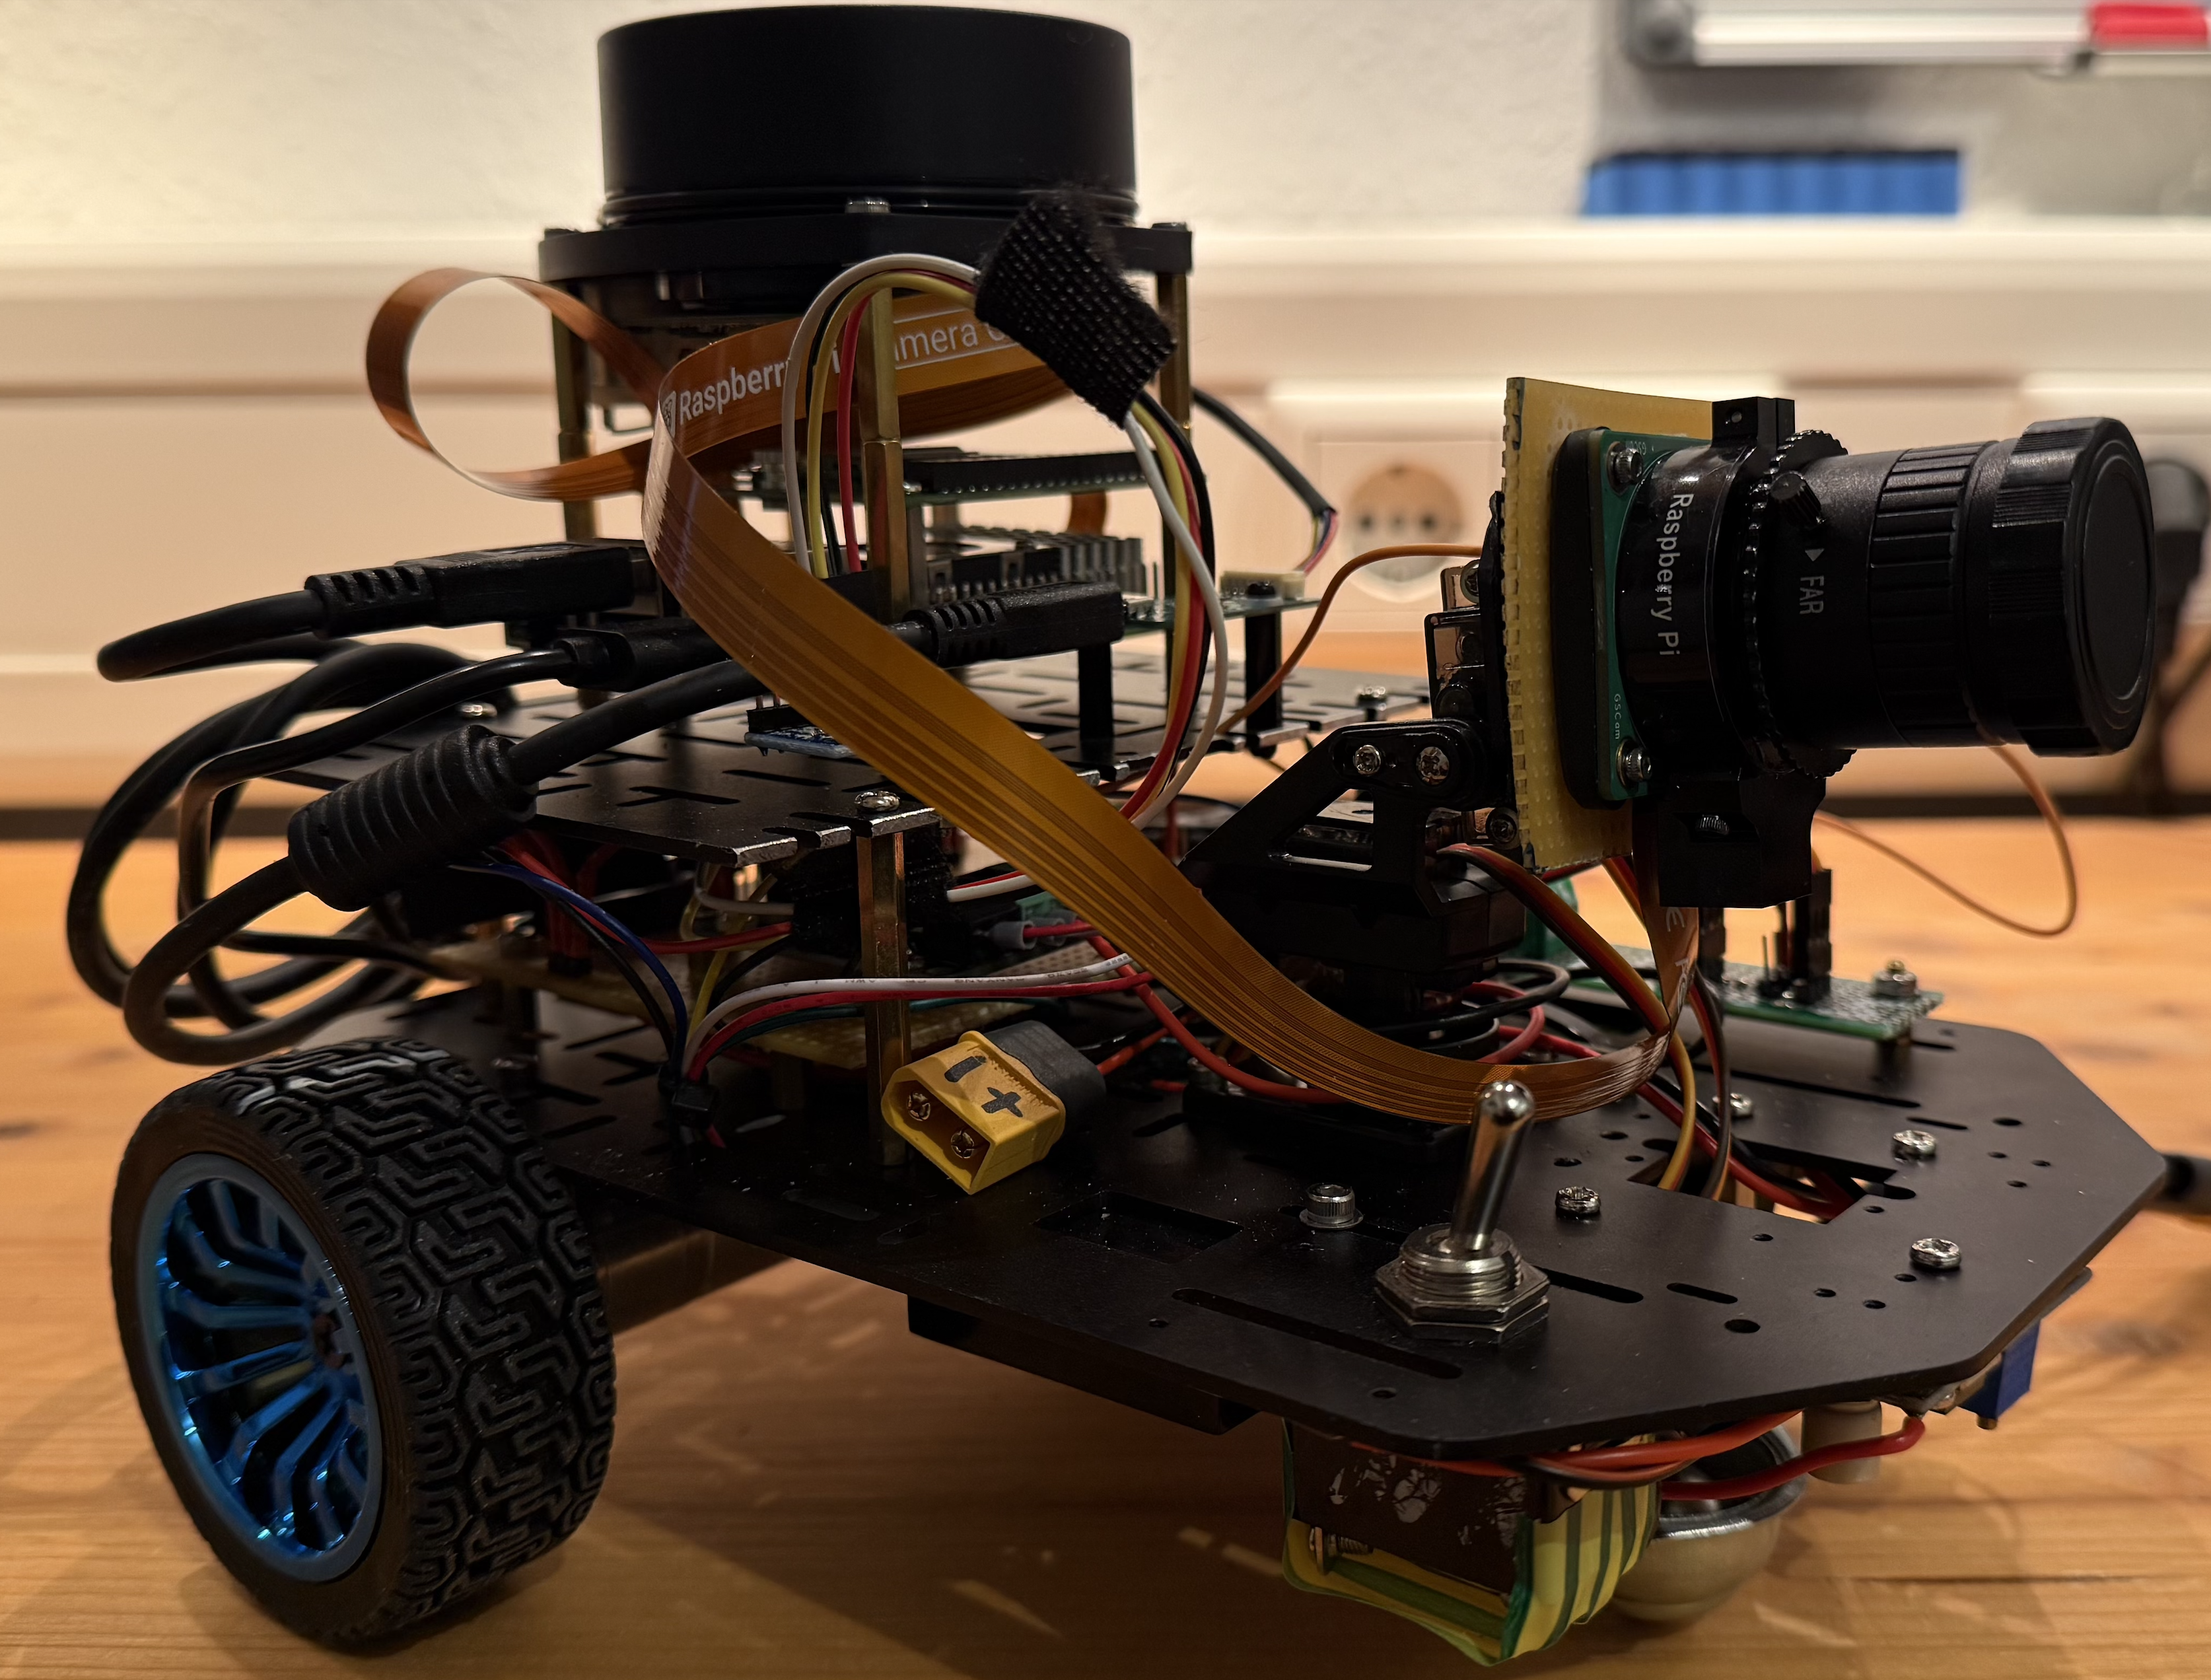
\includegraphics[
        width=\linewidth,
        height=9.8cm,
        keepaspectratio,
        % optional: Rover größer, weniger Hintergrund:
        trim=0 120 0 60,clip
      ]{images/cover.jpg}
    }{
      \IfFileExists{images/cover.png}{
        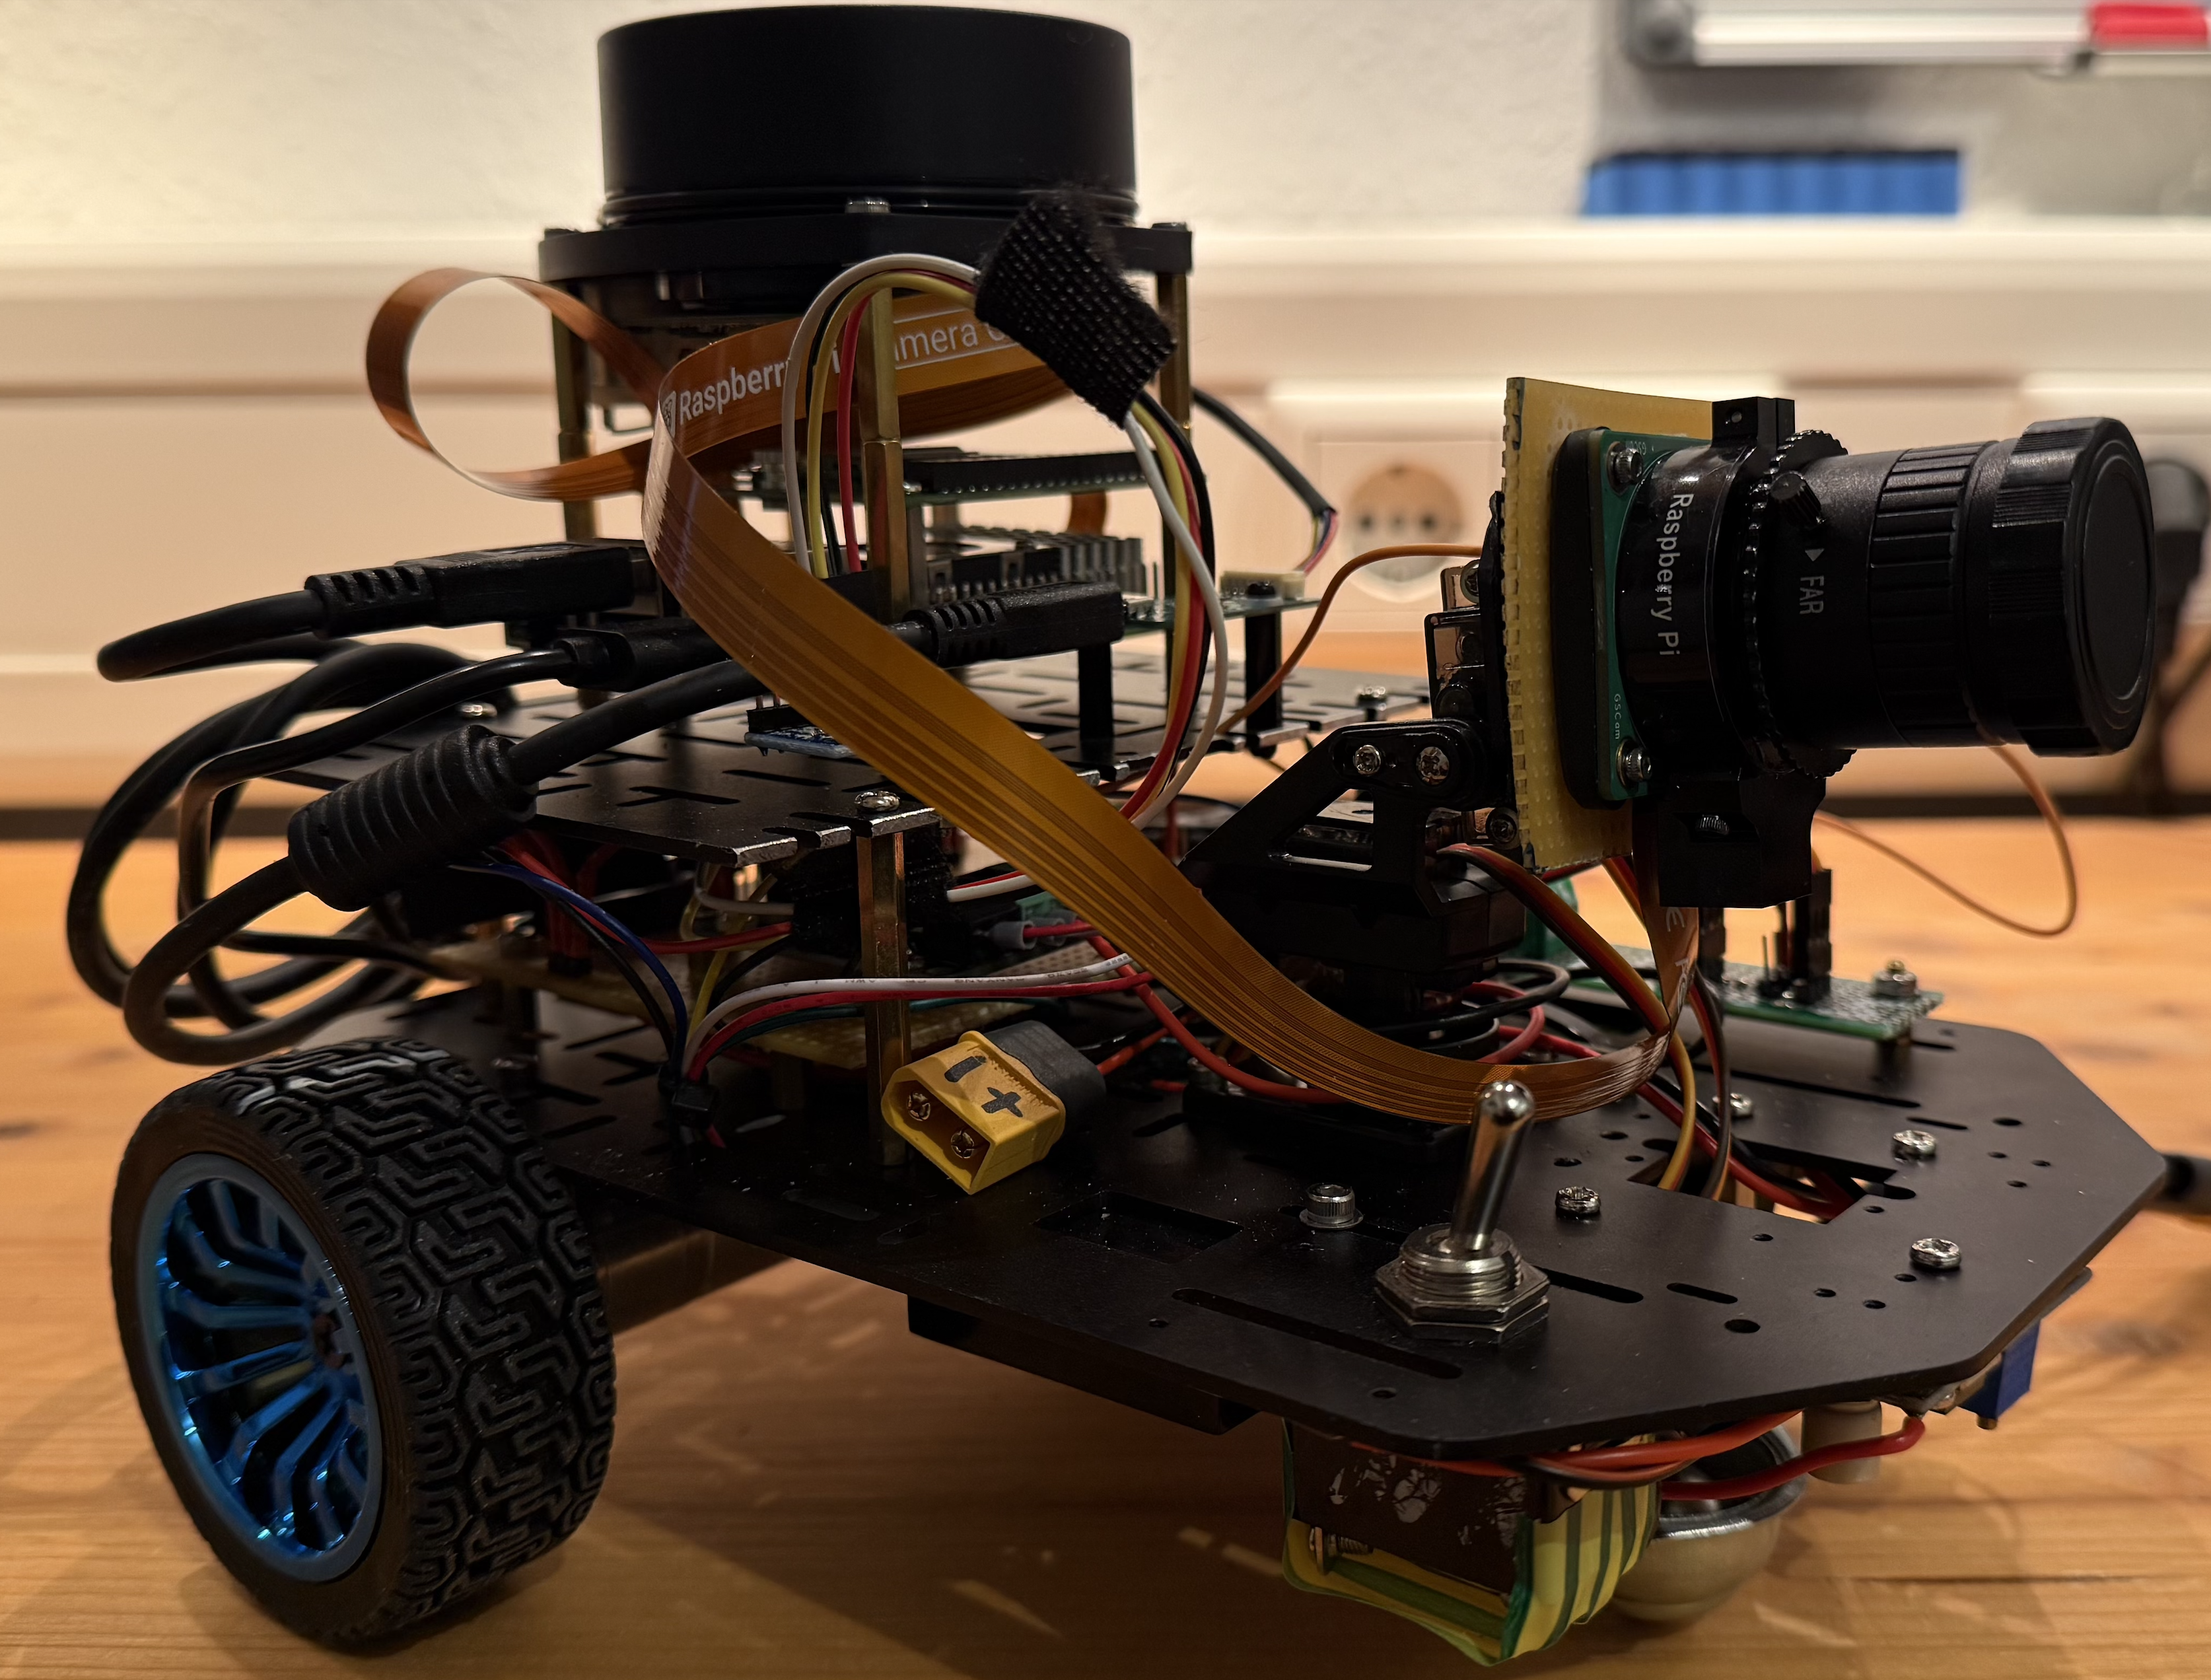
\includegraphics[width=\linewidth,height=9.8cm,keepaspectratio]{images/cover.png}
      }{
        \sffamily\Large cover.{jpg,png} fehlt
      }
    }
  \end{tcolorbox}

  \vspace{0.45cm}

  \begin{tcolorbox}[
    colback=white,
    colframe=arduinoblue!65,
    arc=0mm,
    boxrule=0.6pt,
    width=\CoverW,
    boxsep=4pt
  ]
    \centering\sffamily
    \textbf{Technologie-Stack}\par
    \vspace{0.35em}
    {\small \DocStack\par}
  \end{tcolorbox}

  \vfill

  {\footnotesize\sffamily
  \begin{tabular*}{\CoverW}{@{\extracolsep{\fill}} l r}
    Stand: \today & Jan Unger\\
    AMR-Projekt & Version: \DocVersion\\
  \end{tabular*}\par
  }
\end{titlepage}




\pagenumbering{roman}

% Inhaltsverzeichnis: bewusst ohne Fancy-Header (ruhiger Master-Look)
\begingroup
  \pagestyle{plain}
  \tableofcontents
\endgroup
\clearpage

\pagenumbering{arabic}

% =============================================================================
% Inhalte einbinden (content/*.tex)
% =============================================================================

% =====================================================================
% Phase 1 – micro-ROS auf ESP32-S3 (USB-Serial)
% Quelle: 01-microros-esp32s3.md (v3.2.0, updated 2025-12-20)
% =====================================================================

\section{Phase 1: micro-ROS auf ESP32-S3 (USB-Serial)}

\begin{infobox}[Status \& Version]
\begin{itemize}
  \item Status: \textbf{completed}
  \item Updated: \textbf{2025-12-20}
  \item Version: \textbf{3.2.0}
  \item Source: \filep{firmware/src/main.cpp}, \filep{firmware/include/config.h}, \filep{firmware/platformio.ini}
\end{itemize}
\end{infobox}

\subsection{Zielbild \& Definition of Done}

\textbf{Zielbild:}
\begin{itemize}
  \item ESP32-S3 läuft als \textbf{micro-ROS Client} über \textbf{USB-CDC (Serial)}.
  \item \topic{/cmd\_vel} steuert Motoren über \textbf{Cytron MDD3A Dual-PWM}.
  \item \topic{/odom\_raw} wird publiziert (\texttt{geometry\_msgs/Pose2D}) und ist plausibel.
  \item \textbf{Failsafe} stoppt Motoren nach \texttt{FAILSAFE\_TIMEOUT\_MS = 2000}.
\end{itemize}

\textbf{DoD (verifiziert 2025-12-20):}
\begin{itemize}[label=\(\checkmark\)]
  \item Agent verbindet stabil (Reconnect reproduzierbar).
  \item \topic{/cmd\_vel} wirkt (vor/zurück/rotieren).
  \item \topic{/odom\_raw} plausibel (\(x\) steigt vorwärts, \(\theta\) bei Drehung).
  \item Timeout-Failsafe stoppt deterministisch nach \(\approx \SI{2}{\second}\).
  \item \topic{/esp32/heartbeat} läuft (\(\approx \SI{1}{\hertz}\)).
\end{itemize}

\subsection{Testergebnisse (2025-12-20)}

\begin{table}[H]
\centering
\begin{tabularx}{\textwidth}{@{} l X X c @{}}
\toprule
\textbf{Test} & \textbf{Befehl} & \textbf{Ergebnis} & \textbf{Status} \\
\midrule
Agent-Verbindung & -- & \texttt{fd: 3} stabil & \(\checkmark\) \\
Heartbeat & \texttt{ros2 topic echo /esp32/heartbeat} & \(\approx \SI{1}{\hertz}\) & \(\checkmark\) \\
Vorwärts & \texttt{linear.x: 0.15} & Räder drehen vorwärts & \(\checkmark\) \\
Rückwärts & \texttt{linear.x: -0.15} & Räder drehen rückwärts & \(\checkmark\) \\
Drehen links & \texttt{angular.z: 0.5} & Roboter dreht links & \(\checkmark\) \\
Drehen rechts & \texttt{angular.z: -0.5} & Roboter dreht rechts & \(\checkmark\) \\
Failsafe & Ctrl+C, \(\SI{2}{\second}\) warten & Motoren stoppen & \(\checkmark\) \\
Odom & \texttt{ros2 topic echo /odom\_raw} & \(x,y,\theta\) plausibel & \(\checkmark\) \\
\bottomrule
\end{tabularx}
\end{table}

\textbf{Odom-Beispiel nach Testfahrt:}
\begin{lstlisting}[style=shell]
x: 0.899
y: -0.329
theta: 6.09
\end{lstlisting}

\subsection{Systemübersicht}

\begin{figure}[H]
  \centering
  \includegraphics[width=0.92\textwidth]{images/Architektur.png}
  \caption{Phase-1-Architektur (micro-ROS über USB-Serial): Der ESP32-S3 arbeitet als micro-ROS-Client und führt auf Core~0 die Regel-/Odometrie-Schleife (\(\SI{100}{\hertz}\)) inkl. Failsafe (\(\SI{2}{\second}\) Timeout) aus, während Core~1 die micro-ROS-Kommunikation bedient. Über USB-CDC bei \(\SI{921600}{\baud}\) ist der Raspberry~Pi~5 (Docker) mit dem \texttt{micro-ros-agent} verbunden; im ROS~2-Workspace werden Topics wie \topic{/cmd\_vel} (Motorsteuerung) und \topic{/odom\_raw} (Pose2D) getestet/überwacht.}
  \label{fig:architektur}
\end{figure}



\subsection{Topics (verifiziert)}

\begin{table}[H]
\centering
\begin{tabularx}{\textwidth}{@{} l l l X @{}}
\toprule
\textbf{Topic} & \textbf{Typ} & \textbf{Richtung} & \textbf{Funktion} \\
\midrule
\topic{/cmd\_vel} & \texttt{geometry\_msgs/Twist} & Sub & Geschwindigkeitsbefehle \\
\topic{/odom\_raw} & \texttt{geometry\_msgs/Pose2D} & Pub & Odometrie (\(x,y,\theta\)) \\
\topic{/esp32/heartbeat} & \texttt{std\_msgs/Int32} & Pub & Lebenszeichen \\
\topic{/esp32/led\_cmd} & \texttt{std\_msgs/Bool} & Sub & LED-Steuerung \\
\bottomrule
\end{tabularx}
\end{table}

\subsection{Hardware (Phase 1)}

\begin{table}[H]
\centering
\begin{tabularx}{\textwidth}{@{} l X X @{}}
\toprule
\textbf{Komponente} & \textbf{Spezifikation} & \textbf{Rolle} \\
\midrule
Seeed XIAO ESP32-S3 & Dual-Core Xtensa LX7, USB-CDC & micro-ROS Client + Control \\
Cytron MDD3A & Dual-PWM, \(\SIrange{4}{16}{\volt}\) & Motortreiber \\
JGA25-370 (2×) & \(\SI{12}{\volt}\) DC + Hall-Encoder & Antrieb + Odometrie \\
Raspberry Pi 5 & ROS 2 Humble (Docker) & micro-ROS Agent + Host \\
\bottomrule
\end{tabularx}
\end{table}

\subsubsection{Pin-Mapping}

\begin{table}[H]
\centering
\begin{tabularx}{\textwidth}{@{} l l l X @{}}
\toprule
\textbf{Funktion} & \textbf{Pin} & \textbf{Typ} & \textbf{Hinweis} \\
\midrule
Motor Left A & \pin{D0} & PWM & \(\rightarrow\) PWM\_CH 1 (getauscht) \\
Motor Left B & \pin{D1} & PWM & \(\rightarrow\) PWM\_CH 0 (getauscht) \\
Motor Right A & \pin{D2} & PWM & \(\rightarrow\) PWM\_CH 3 (getauscht) \\
Motor Right B & \pin{D3} & PWM & \(\rightarrow\) PWM\_CH 2 (getauscht) \\
Encoder Left A & \pin{D6} & IRQ & A-only \\
Encoder Right A & \pin{D7} & IRQ & A-only \\
LED/MOSFET & \pin{D10} & GPIO & Status \\
\bottomrule
\end{tabularx}
\end{table}

\begin{tipbox}[Hinweis]
Die PWM-Kanäle wurden getauscht (A\(\leftrightarrow\)B), um die korrekte Fahrtrichtung zu erreichen.
\end{tipbox}

\subsection{Firmware – Parameter (v3.2.0)}

\subsubsection{config.h}

\begin{table}[H]
\centering
\begin{tabularx}{\textwidth}{@{} l l X @{}}
\toprule
\textbf{Parameter} & \textbf{Wert} & \textbf{Beschreibung} \\
\midrule
\texttt{LOOP\_RATE\_HZ} & \(\SI{100}{\hertz}\) & Control-Zyklus (\(\SI{10}{\milli\second}\)) \\
\texttt{ODOM\_PUBLISH\_HZ} & \(\SI{20}{\hertz}\) & Odom Publish (\(\SI{50}{\milli\second}\)) \\
\texttt{FAILSAFE\_TIMEOUT\_MS} & \(\SI{2000}{\milli\second}\) & Heartbeat-Timeout \\
\texttt{MOTOR\_PWM\_FREQ} & \(\SI{20}{\kilo\hertz}\) & PWM-Frequenz (unhörbar) \\
\texttt{MOTOR\_PWM\_BITS} & \(\SI{8}{}\) & Auflösung (0–255) \\
\texttt{PWM\_DEADZONE} & \(\SI{35}{}\) & Mindest-PWM \\
\texttt{WHEEL\_DIAMETER} & \(\SI{0.065}{\meter}\) & Raddurchmesser \\
\texttt{WHEEL\_BASE} & \(\SI{0.178}{\meter}\) & Spurbreite \\
\bottomrule
\end{tabularx}
\end{table}

\subsubsection{PWM-Kanäle (getauscht für korrekte Richtung)}

\begin{lstlisting}[style=arduino,caption={PWM-Channel Mapping (A/B getauscht)}]
#define PWM_CH_LEFT_A  1  // war 0
#define PWM_CH_LEFT_B  0  // war 1
#define PWM_CH_RIGHT_A 3  // war 2
#define PWM_CH_RIGHT_B 2  // war 3
\end{lstlisting}

\subsubsection{Regelung (Open-Loop mit Feedforward)}

\begin{table}[H]
\centering
\begin{tabularx}{\textwidth}{@{} l l X @{}}
\toprule
\textbf{Parameter} & \textbf{Wert} & \textbf{Beschreibung} \\
\midrule
\texttt{PID\_KP} & \(\SI{0.0}{}\) & Deaktiviert \\
\texttt{PID\_KI} & \(\SI{0.0}{}\) & Deaktiviert \\
\texttt{PID\_KD} & \(\SI{0.0}{}\) & Deaktiviert \\
\texttt{feedforward\_gain} & \(\SI{2.0}{}\) & Direkte Ansteuerung \\
\bottomrule
\end{tabularx}
\end{table}

\begin{warnbox}[Hinweis]
PID wurde deaktiviert, da die Encoder-Polarität invertiert ist. Feedforward ermöglicht stabile Open-Loop-Steuerung. PID-Tuning ist sinnvoll ab Phase 4+, nachdem die Encoder-Richtungsheuristik validiert ist.
\end{warnbox}

\subsubsection{main.cpp – Feedforward-Berechnung}

\begin{lstlisting}[style=arduino,caption={Feedforward + (optional) PID}]
float feedforward_gain = 2.0f;
float pwm_l = feedforward_gain * set_v_l + pid_left.compute(set_v_l, v_enc_l, dt);
float pwm_r = feedforward_gain * set_v_r + pid_right.compute(set_v_r, v_enc_r, dt);

// Begrenzen auf PWM-Bereich
pwm_l = constrain(pwm_l, -1.0f, 1.0f);
pwm_r = constrain(pwm_r, -1.0f, 1.0f);
\end{lstlisting}

\subsection{Build/Flash/Monitor (PlatformIO)}

\subsubsection{Firmware kompilieren und flashen (Mac)}

\begin{lstlisting}[style=shell]
cd ~/daten/start/IoT/AMR/amr-platform/firmware
pio run -e seeed_xiao_esp32s3 -t upload
\end{lstlisting}

\subsubsection{Serial Monitor (Debug)}

\begin{lstlisting}[style=shell]
pio device monitor -b 921600
\end{lstlisting}

\subsection{Docker-Setup (Pi 5)}

\subsubsection{docker-compose.yml (Auszug)}

\begin{lstlisting}[style=shell]
services:
  microros_agent:
    image: microros/micro-ros-agent:humble
    container_name: amr_agent
    network_mode: host
    privileged: true
    restart: always
    command: serial --dev /dev/ttyACM0 -b 921600
    devices:
      - /dev/ttyACM0:/dev/ttyACM0

  amr_dev:
    build: .
    container_name: amr_base
    network_mode: host
    privileged: true
    volumes:
      - ../ros2_ws:/root/ros2_ws
    command: tail -f /dev/null
\end{lstlisting}

\subsubsection{Container starten}

\begin{lstlisting}[style=shell]
cd ~/amr-platform/docker
docker compose up -d
docker compose ps
\end{lstlisting}

\subsubsection{Agent-Logs prüfen}

\begin{lstlisting}[style=shell]
docker compose logs microros_agent --tail 10
\end{lstlisting}

\textbf{Erwartete Ausgabe:}
\begin{lstlisting}[style=shell]
amr_agent | [timestamp] info | TermiosAgentLinux.cpp | init | running... | fd: 3
\end{lstlisting}

\subsection{Smoke-Tests}

\subsubsection{1) In Container gehen}

\begin{lstlisting}[style=shell]
docker compose exec amr_dev bash
source /opt/ros/humble/setup.bash
\end{lstlisting}

\subsubsection{2) Topics prüfen}

\begin{lstlisting}[style=shell]
ros2 topic list
\end{lstlisting}

\textbf{Erwartung:}
\begin{lstlisting}[style=shell]
/cmd_vel
/esp32/heartbeat
/esp32/led_cmd
/odom_raw
/parameter_events
/rosout
\end{lstlisting}

\subsubsection{3) Motor-Tests (Räder aufbocken!)}

\begin{warnbox}[Sicherheit]
Vor Motor-Tests Räder aufbocken: der Roboter darf nicht unkontrolliert losfahren.
\end{warnbox}

\begin{lstlisting}[style=shell,caption={Motor-Tests via \texttt{\detokenize{/cmd_vel}}}]
# Vorwärts
ros2 topic pub /cmd_vel geometry_msgs/msg/Twist \
  "{linear: {x: 0.15}, angular: {z: 0.0}}" -r 10

# Rückwärts (Ctrl+C, dann:)
ros2 topic pub /cmd_vel geometry_msgs/msg/Twist \
  "{linear: {x: -0.15}, angular: {z: 0.0}}" -r 10

# Drehen links
ros2 topic pub /cmd_vel geometry_msgs/msg/Twist \
  "{linear: {x: 0.0}, angular: {z: 0.5}}" -r 10

# Drehen rechts
ros2 topic pub /cmd_vel geometry_msgs/msg/Twist \
  "{linear: {x: 0.0}, angular: {z: -0.5}}" -r 10
\end{lstlisting}

\subsubsection{4) Failsafe-Test}

\begin{enumerate}
  \item Motor-Befehl senden (Räder drehen)
  \item \texttt{Ctrl+C} drücken
  \item \(\SI{2}{\second}\) warten
  \item \textbf{Erwartung:} Motoren stoppen automatisch
\end{enumerate}

\subsubsection{5) Odometrie prüfen}

\begin{lstlisting}[style=shell]
ros2 topic echo /odom_raw --once
\end{lstlisting}

\subsection{Troubleshooting}

\begin{table}[H]
\centering
\begin{tabularx}{\textwidth}{@{} X X X @{}}
\toprule
\textbf{Problem} & \textbf{Ursache} & \textbf{Lösung} \\
\midrule
\texttt{Serial port not found} & ESP32 nicht angeschlossen & USB-Kabel prüfen, \texttt{ls /dev/ttyACM*} \\
Topics fehlen & Agent nicht verbunden & Agent-Logs prüfen, ESP32 Reset \\
Räder drehen falsche Richtung & PWM-Kanäle falsch & A\(\leftrightarrow\)B tauschen in \texttt{config.h} \\
Motor reagiert nicht & Feedforward zu niedrig & \texttt{feedforward\_gain} erhöhen \\
PID eskaliert & Encoder-Polarität invertiert & PID deaktivieren (\(\texttt{Kp}=0\)) \\
Failsafe greift nicht & Timeout zu kurz & \texttt{FAILSAFE\_TIMEOUT\_MS} erhöhen \\
\bottomrule
\end{tabularx}
\end{table}

\subsection{Bekannte Einschränkungen}

\begin{enumerate}
  \item \textbf{Open-Loop-Steuerung:} PID deaktiviert, keine Geschwindigkeitsregelung.
  \item \textbf{Encoder A-only:} Richtung wird aus Soll-Geschwindigkeit abgeleitet.
  \item \textbf{Odom-Rate:} effektiv \(\approx \SIrange{3}{6}{\hertz}\) durch Serial-Transport.
\end{enumerate}

\subsection{Nächste Schritte}

\begin{table}[H]
\centering
\begin{tabularx}{\textwidth}{@{} l X l @{}}
\toprule
\textbf{Phase} & \textbf{Beschreibung} & \textbf{Status} \\
\midrule
Phase 1 & micro-ROS ESP32-S3 & abgeschlossen \\
Phase 2 & Docker-Infrastruktur & vorhanden \\
Phase 3 & RPLidar A1 Integration (\filep{/dev/ttyUSB0}) & bereit \\
Phase 4 & EKF Sensor Fusion & offen \\
Phase 5 & SLAM (\texttt{slam\_toolbox}) & offen \\
Phase 6 & Nav2 autonome Navigation & offen \\
\bottomrule
\end{tabularx}
\end{table}

\subsection{Changelog}

\begin{table}[H]
\centering
\begin{tabularx}{\textwidth}{@{} l l X @{}}
\toprule
\textbf{Version} & \textbf{Datum} & \textbf{Änderungen} \\
\midrule
v1.0 & 2025-12-19 & Initiale Dokumentation \\
v3.1.0 & 2025-12-20 & PID aktiviert, Baudrate \(\SI{921600}{\baud}\) \\
v3.2.0 & 2025-12-20 & PWM-Kanäle getauscht, Feedforward (Gain=\(\SI{2.0}{}\)), PID deaktiviert, alle Tests bestanden \\
\bottomrule
\end{tabularx}
\end{table}

% =============================================================================
% Phase 1 – Befehlsreferenz
% (Fragment ohne Präambel; setzt Listings/Boxen-Stile aus main.tex voraus)
% =============================================================================

\section{Phase 1 – Befehlsreferenz}
\label{sec:phase1-befehle}

\begin{infobox}[Zweck]
Schnelle Befehls-Sammlung für Phase~1 (micro-ROS Agent im Docker auf dem Pi, ESP32 per USB-Serial).
Arbeitsverzeichnis: \filep{\textasciitilde/amr-platform/docker}.
\end{infobox}

\subsection{Nach Pi Reboot}

\begin{lstlisting}[style=shell]
cd ~/amr-platform/docker
docker compose up -d
sleep 5
docker compose logs microros_agent --tail 5
\end{lstlisting}

\begin{cmdbox}[Erwartung]
\ttfamily running... \textbar\ fd: 3
\end{cmdbox}

\subsection{Nach ESP32 Reboot (USB umgesteckt)}

\begin{lstlisting}[style=shell]
cd ~/amr-platform/docker
docker compose restart microros_agent
sleep 5
docker compose logs microros_agent --tail 5
\end{lstlisting}

\begin{cmdbox}[Erwartung]
\ttfamily running... \textbar\ fd: 3
\end{cmdbox}

\subsection{Notfall-Stop (falls Räder drehen)}

\begin{warnbox}[Sicherheit]
Wenn sich der Rover unkontrolliert bewegt: \emph{sofort} Stop senden. Bei Motor-Tests Räder aufbocken.
\end{warnbox}

\begin{lstlisting}[style=shell]
docker compose exec amr_dev bash -c "source /opt/ros/humble/setup.bash && \
  ros2 topic pub --once /cmd_vel geometry_msgs/msg/Twist '{linear: {x: 0.0}, angular: {z: 0.0}}'"
\end{lstlisting}

\subsection{Smoke-Tests}

\subsubsection{1. In Container gehen}

\begin{lstlisting}[style=shell]
docker compose exec amr_dev bash
source /opt/ros/humble/setup.bash
\end{lstlisting}

\subsubsection{2. Topics prüfen}

\begin{lstlisting}[style=shell]
ros2 topic list
\end{lstlisting}

\begin{cmdbox}[Erwartung]
\ttfamily
/cmd\_vel\\
/esp32/heartbeat\\
/esp32/led\_cmd\\
/odom\_raw\\
/parameter\_events\\
/rosout
\end{cmdbox}

\subsubsection{3. Heartbeat prüfen}

\begin{lstlisting}[style=shell]
ros2 topic echo /esp32/heartbeat
\end{lstlisting}

\begin{tipbox}[Erwartung]
Counter inkrementiert ca. $1\times/\mathrm{s}$ (mit \texttt{Ctrl+C} beenden).
\end{tipbox}

\subsubsection{4. Odometrie prüfen}

\begin{lstlisting}[style=shell]
ros2 topic echo /odom_raw --once
\end{lstlisting}

\begin{tipbox}[Erwartung]
Ausgabe enthält plausible \texttt{x}, \texttt{y}, \texttt{theta} Werte.
\end{tipbox}

\subsubsection{5. Frequenzen messen}

\begin{lstlisting}[style=shell]
ros2 topic hz /esp32/heartbeat
\end{lstlisting}

\begin{lstlisting}[style=shell]
ros2 topic hz /odom_raw
\end{lstlisting}

\begin{tipbox}[Erwartung]
Heartbeat $\approx \SI{1}{\hertz}$, Odom $\approx \SIrange{3}{6}{\hertz}$.
\end{tipbox}

\subsection{Motor-Tests}

\begin{warnbox}[Sicherheit]
Räder aufbocken (kein Bodenkontakt). Notfall-Stop bereithalten.
\end{warnbox}

\subsubsection{Vorwärts}

\begin{lstlisting}[style=shell]
ros2 topic pub /cmd_vel geometry_msgs/msg/Twist \
  "{linear: {x: 0.15}, angular: {z: 0.0}}" -r 10
\end{lstlisting}

\subsubsection{Rückwärts}

\begin{lstlisting}[style=shell]
ros2 topic pub /cmd_vel geometry_msgs/msg/Twist \
  "{linear: {x: -0.15}, angular: {z: 0.0}}" -r 10
\end{lstlisting}

\subsubsection{Drehen links}

\begin{lstlisting}[style=shell]
ros2 topic pub /cmd_vel geometry_msgs/msg/Twist \
  "{linear: {x: 0.0}, angular: {z: 0.5}}" -r 10
\end{lstlisting}

\subsubsection{Drehen rechts}

\begin{lstlisting}[style=shell]
ros2 topic pub /cmd_vel geometry_msgs/msg/Twist \
  "{linear: {x: 0.0}, angular: {z: -0.5}}" -r 10
\end{lstlisting}

\subsubsection{Manueller Stop}

\begin{lstlisting}[style=shell]
ros2 topic pub --once /cmd_vel geometry_msgs/msg/Twist \
  "{linear: {x: 0.0}, angular: {z: 0.0}}"
\end{lstlisting}

\begin{tipbox}[Hinweis]
Nach \texttt{Ctrl+C} stoppt der Failsafe die Motoren automatisch nach ca. \SI{2}{\second}.
\end{tipbox}

\subsection{Failsafe-Test}

\begin{enumerate}
  \item Motor-Befehl senden (Räder drehen).
  \item \texttt{Ctrl+C} drücken.
  \item \SI{2}{\second} warten.
  \item \textbf{Erwartung:} Motoren stoppen automatisch.
\end{enumerate}

\subsection{Odom nach Fahrt prüfen}

\begin{lstlisting}[style=shell]
ros2 topic echo /odom_raw --once
\end{lstlisting}

\begin{tipbox}[Erwartung]
Nach Vorwärtsfahrt: \texttt{x} $> 0$. Nach Drehung: \texttt{theta} ändert sich.
\end{tipbox}

\subsection{Checkliste Phase 1}

\begin{table}[H]
\centering
\begin{tabularx}{\textwidth}{@{}lXc@{}}
\toprule
\textbf{Test} & \textbf{Erwartung} & \textbf{Status} \\
\midrule
Agent verbindet & \texttt{fd: 3} & $\square$ \\
Topics vorhanden & 6 Topics & $\square$ \\
Heartbeat & $\approx \SI{1}{\hertz}$ & $\square$ \\
Odom publiziert & \texttt{x, y, theta} Werte & $\square$ \\
Vorwärts & Räder drehen vorwärts & $\square$ \\
Rückwärts & Räder drehen rückwärts & $\square$ \\
Drehen links & Roboter dreht links & $\square$ \\
Drehen rechts & Roboter dreht rechts & $\square$ \\
Failsafe & Stop nach \SI{2}{\second} & $\square$ \\
\bottomrule
\end{tabularx}
\end{table}

\subsection{Troubleshooting}

\begin{table}[H]
\centering
\begin{tabularx}{\textwidth}{@{}lX@{}}
\toprule
\textbf{Problem} & \textbf{Lösung} \\
\midrule
\texttt{Serial port not found} & USB-Kabel prüfen, \texttt{ls /dev/ttyACM*} \\
Topics fehlen & \texttt{docker compose restart microros\_agent} \\
Räder reagieren nicht & Feedforward-Gain prüfen (2.0) \\
Falsches Verhalten & USB ziehen, Firmware prüfen \\
\bottomrule
\end{tabularx}
\end{table}

% =====================================================================
% Phase 2 – ROS 2 Humble auf Pi 5 via Docker + micro-ROS Agent
% Fragment ohne Präambel (setzt Styles/Makros aus main.tex voraus)
% =====================================================================

\section{Phase 2: ROS 2 Humble auf Raspberry Pi 5 (Docker) + micro-ROS Agent}
\label{sec:phase2-ros2-humble-docker-pi5}

\begin{infobox}[Status \& Version]
\begin{itemize}
  \item Status: \textbf{completed}
  \item Updated: \textbf{2025-12-20}
  \item Version: \textbf{2.0}
  \item Depends on: \textbf{Phase 1 (micro-ROS auf ESP32-S3)}
  \item Next: \textbf{Phase 3 (RPLidar A1)}
\end{itemize}
\end{infobox}

\subsection{Zielbild \& Definition of Done}

\subsubsection{Zielbild}
\begin{itemize}
  \item Raspberry Pi 5 (Raspberry Pi OS \textbf{64-bit}) betreibt \textbf{ROS 2 Humble} in \textbf{Docker}.
  \item micro-ROS Agent läuft reproduzierbar (Container) und verbindet sich über \textbf{USB-Serial} zum ESP32-S3.
  \item Host-ROS kann:
  \begin{itemize}
    \item \topic{/cmd\_vel} publizieren \(\rightarrow\) Motor reagiert
    \item \topic{/odom\_raw} empfangen \(\rightarrow\) Werte plausibel
    \item \topic{/esp32/heartbeat} empfangen \(\rightarrow\) Agent-Verbindung verifiziert
  \end{itemize}
\end{itemize}

\subsubsection{DoD (verifiziert 2025-12-20)}
\begin{itemize}[label=\(\checkmark\)]
  \item \texttt{docker compose up} startet Container ohne manuelle Nacharbeit.
  \item Agent verbindet stabil über \filep{/dev/ttyACM0} mit $921600\,\mathrm{Bd}$.
  \item ROS Smoke-Tests sind grün:
  \begin{itemize}[label=\(\checkmark\)]
    \item \texttt{ros2 topic list} zeigt \topic{/cmd\_vel}, \topic{/odom\_raw}, \topic{/esp32/heartbeat}, \topic{/esp32/led\_cmd}
    \item \texttt{ros2 topic pub /cmd\_vel ...} bewegt den Rover
    \item \texttt{ros2 topic echo /odom\_raw} liefert kontinuierliche Werte
  \end{itemize}
  \item Failsafe stoppt Motoren nach \SI{2}{\second} Timeout.
\end{itemize}

\subsection{Docker-Images (Regel)}

\begin{table}[H]
\centering
\begin{tabularx}{\textwidth}{@{} l l X @{}}
\toprule
\textbf{Service / Container} & \textbf{Image} & \textbf{Funktion} \\
\midrule
\texttt{microros\_agent} / \texttt{amr\_agent} & \texttt{microros/micro-ros-agent:humble} & Serial Agent \\
\texttt{amr\_dev} / \texttt{amr\_base} & Custom (ROS 2 Humble) & Workspace \\
\bottomrule
\end{tabularx}
\end{table}

\textbf{Warum Humble statt Jazzy:}
\begin{itemize}
  \item micro-ROS Agent für Humble stabiler auf \texttt{arm64}
  \item Kompatibilität mit bestehenden Packages (Nav2, \texttt{slam\_toolbox})
\end{itemize}

\subsection{Host-Voraussetzungen}

\subsubsection{System}
\begin{itemize}
  \item Raspberry Pi 5, Raspberry Pi OS \textbf{64-bit} (Bookworm)
  \item Docker Engine + Docker Compose Plugin
\end{itemize}

\subsubsection{USB-Serial prüfen}
\begin{lstlisting}[style=shell]
ls -l /dev/ttyACM*
# Erwartung: /dev/ttyACM0 (ESP32-S3)

ls -l /dev/ttyUSB*
# Erwartung: /dev/ttyUSB0 (RPLidar A1)
\end{lstlisting}

\subsection{Repo-Struktur}

\begin{figure}[H]
  \centering
  \includegraphics[width=0.4\textwidth]{images/projekt-struktur.png}
  \caption{Projektstruktur des Repositories \texttt{amr-platform}: \texttt{firmware/} enthält die ESP32-S3-Firmware (PlatformIO mit \texttt{src/main.cpp} und \texttt{include/config.h}), \texttt{ros2\_ws/src/} den ROS~2-Workspace mit Paketen für Bridge/Bringup/Description sowie \texttt{sllidar\_ros2}. Die Laufzeitumgebung ist in \texttt{docker/} (Dockerfile, Compose, Entrypoint) gekapselt. Automatisierung und Betrieb liegen in \texttt{scripts/} (Deployment, micro-ROS-Agent-Service, Dokumentations-Converter). \texttt{docs/} bündelt Projektdokumentation; \texttt{README.md}, \texttt{LICENSE}, \texttt{start.html} und \texttt{main-design.css} bilden Einstieg und Styling der Doku.}
  \label{fig:projektstruktur}
\end{figure}


\subsection{Docker Compose}

\subsubsection{docker-compose.yml}
\begin{lstlisting}[style=shell]
services:
  microros_agent:
    image: microros/micro-ros-agent:humble
    container_name: amr_agent
    network_mode: host
    privileged: true
    restart: always
    command: serial --dev /dev/ttyACM0 -b 921600
    devices:
      - /dev/ttyACM0:/dev/ttyACM0

  amr_dev:
    build: .
    container_name: amr_base
    network_mode: host
    privileged: true
    volumes:
      - ../ros2_ws:/root/ros2_ws
    command: tail -f /dev/null
\end{lstlisting}

\subsubsection{Dockerfile}
\begin{lstlisting}[style=shell]
FROM ros:humble-ros-base

RUN apt-get update && apt-get install -y \
    python3-colcon-common-extensions \
    ros-humble-tf2-tools \
    ros-humble-xacro \
    ros-humble-rviz2 \
    && rm -rf /var/lib/apt/lists/*

WORKDIR /root/ros2_ws
\end{lstlisting}

\subsection{Befehle}

\subsubsection{Nach Pi Reboot}
\begin{lstlisting}[style=shell]
cd ~/amr-platform/docker
docker compose up -d
sleep 5
docker compose logs microros_agent --tail 5
\end{lstlisting}

\begin{cmdbox}[Erwartung]
\ttfamily running... \textbar\ fd: 3
\end{cmdbox}

\subsubsection{Nach ESP32 Reboot}
\begin{lstlisting}[style=shell]
docker compose restart microros_agent
sleep 5
docker compose logs microros_agent --tail 5
\end{lstlisting}

\subsubsection{In Container gehen}
\begin{lstlisting}[style=shell]
docker compose exec amr_dev bash
source /opt/ros/humble/setup.bash
\end{lstlisting}

\subsection{Smoke-Tests}

\subsubsection{Topics prüfen}
\begin{lstlisting}[style=shell]
ros2 topic list
\end{lstlisting}

\begin{cmdbox}[Erwartung]
\ttfamily
/cmd\_vel\\
/esp32/heartbeat\\
/esp32/led\_cmd\\
/odom\_raw\\
/parameter\_events\\
/rosout
\end{cmdbox}

\subsubsection{Heartbeat}
\begin{lstlisting}[style=shell]
ros2 topic echo /esp32/heartbeat
\end{lstlisting}

\begin{tipbox}[Erwartung]
Counter steigt ca. $\SI{1}{\hertz}$.
\end{tipbox}

\subsubsection{Odometrie}
\begin{lstlisting}[style=shell]
ros2 topic echo /odom_raw --once
\end{lstlisting}

\begin{tipbox}[Erwartung]
Ausgabe enthält plausible \texttt{x}, \texttt{y}, \texttt{theta}.
\end{tipbox}

\subsubsection{Motor-Test (Räder aufbocken!)}
\begin{warnbox}[Sicherheit]
Motor-Tests nur mit aufgebockten Rädern (kein Bodenkontakt).
\end{warnbox}

\begin{lstlisting}[style=shell]
# Vorwärts
ros2 topic pub /cmd_vel geometry_msgs/msg/Twist \
  "{linear: {x: 0.15}, angular: {z: 0.0}}" -r 10

# Ctrl+C -> Failsafe stoppt nach 2s
\end{lstlisting}

\subsection{Troubleshooting}

\begin{table}[H]
\centering
\begin{tabularx}{\textwidth}{@{} X X X @{}}
\toprule
\textbf{Problem} & \textbf{Ursache} & \textbf{Lösung} \\
\midrule
Agent sieht ESP32 nicht & Device-Pfad falsch & \texttt{ls /dev/ttyACM*} prüfen \\
Topics fehlen & Agent nicht verbunden & \texttt{docker compose restart microros\_agent} \\
ROS sieht keine Topics & Domain-ID Mismatch & \texttt{network\_mode: host} nutzen \\
Motor reagiert nicht & Failsafe greift & Timeout prüfen (\SI{2000}{\milli\second}) \\
\bottomrule
\end{tabularx}
\end{table}

\subsection{Verifizierte Konfiguration}

\begin{table}[H]
\centering
\begin{tabularx}{\textwidth}{@{} l l @{}}
\toprule
\textbf{Parameter} & \textbf{Wert} \\
\midrule
ROS-Version & Humble \\
Agent-Image & \texttt{microros/micro-ros-agent:humble} \\
Baudrate & $921600\,\mathrm{Bd}$ \\
Device & \filep{/dev/ttyACM0} \\
Services/Container & \texttt{microros\_agent} (\texttt{amr\_agent}), \texttt{amr\_dev} (\texttt{amr\_base}) \\
Network & host \\
\bottomrule
\end{tabularx}
\end{table}

\subsection{Changelog}

\begin{table}[H]
\centering
\begin{tabularx}{\textwidth}{@{} l l X @{}}
\toprule
\textbf{Version} & \textbf{Datum} & \textbf{Änderungen} \\
\midrule
v2.0 & 2025-12-20 & Humble statt Jazzy, $921600\,\mathrm{Bd}$, Container-Namen aktualisiert, Status: abgeschlossen \\
v1.0 & 2025-12-19 & Initiale Jazzy-Version (überholt) \\
\bottomrule
\end{tabularx}
\end{table}

% =====================================================================
% Phase 3 – RPLidar A1 Integration + /scan
% Fragment ohne Präambel (setzt Styles/Makros aus main.tex voraus)
% =====================================================================

\section{Phase 3: RPLidar A1 Integration (+ \topic{/scan})}
\label{sec:phase3-rplidar-a1}

\begin{infobox}[Status \& Version]
\begin{itemize}
  \item Status: \textbf{completed}
  \item Updated: \textbf{2025-12-20}
  \item Version: \textbf{3.0}
  \item Depends on: Phase 1 (micro-ROS ESP32-S3), Phase 2 (Docker ROS 2 Humble)
  \item Next: Phase 4 (URDF + TF + EKF)
\end{itemize}
\end{infobox}

\subsection{Zielbild \& Definition of Done}

\subsubsection{Zielbild}
\begin{itemize}
  \item RPLidar A1 läuft am Raspberry Pi 5 (Docker/ROS 2 Humble) als Laser-Treiber.
  \item Topic \topic{/scan} (\texttt{sensor\_msgs/msg/LaserScan}) ist stabil und liefert plausible Werte.
  \item \texttt{frame\_id} ist \texttt{laser} (TF-Anbindung an \texttt{base\_link} folgt in Phase 4).
\end{itemize}

\subsubsection{DoD (verifiziert 2025-12-20)}
\begin{itemize}[label=\(\checkmark\)]
  \item \texttt{ros2 topic hz /scan} zeigt stabile Frequenz \(\approx \SI{7.6}{\hertz}\)
  \item \texttt{ros2 topic echo /scan --once} liefert plausible Werte
  \item \texttt{frame\_id}: \texttt{laser}
  \item Scan-Range: \(-\pi\) bis \(+\pi\), \(\SIrange{0.05}{12.0}{\meter}\)
\end{itemize}

\subsection{Hardware-Info (verifiziert)}

\subsubsection{Sensor}
\begin{table}[H]
\centering
\begin{tabularx}{\textwidth}{@{} l X @{}}
\toprule
\textbf{Parameter} & \textbf{Wert} \\
\midrule
Modell & RPLidar A1 \\
S/N & 74A5FA89C7E19EC8BCE499F0FF725670 \\
Firmware & 1.29 \\
Hardware Rev & 7 \\
Scan Mode & Sensitivity \\
Sample Rate & \(\SI{8}{\kilo\hertz}\) \\
\bottomrule
\end{tabularx}
\end{table}

\subsubsection{Gemessene Werte}
\begin{table}[H]
\centering
\begin{tabularx}{\textwidth}{@{} l X @{}}
\toprule
\textbf{Parameter} & \textbf{Wert} \\
\midrule
Frequenz & \(\approx \SI{7.6}{\hertz}\) \\
\texttt{range\_min} & \(\SI{0.05}{\meter}\) \\
\texttt{range\_max} & \(\SI{12.0}{\meter}\) \\
\texttt{angle\_min} & \(-3.14\,\mathrm{rad}\) \\
\texttt{angle\_max} & \(+3.14\,\mathrm{rad}\) \\
\bottomrule
\end{tabularx}
\end{table}

\subsubsection{Anschluss}
\begin{table}[H]
\centering
\begin{tabularx}{\textwidth}{@{} l l X @{}}
\toprule
\textbf{Device} & \textbf{Port} & \textbf{Hinweis} \\
\midrule
RPLidar A1 & \filep{/dev/ttyUSB0} & USB-Adapter: \texttt{cp210x} \\
\bottomrule
\end{tabularx}
\end{table}

\subsection{Docker-Integration}

\begin{warnbox}[Wichtig]
Kein separater \texttt{rplidar}-Container. Das erzeugt Port-Konflikte. RPLidar wird im \texttt{amr\_dev}-Container gestartet.
\end{warnbox}

\subsubsection{docker-compose.yml (relevanter Auszug)}
\begin{lstlisting}[style=shell]
services:
  microros_agent:
    image: microros/micro-ros-agent:humble
    container_name: amr_agent
    network_mode: host
    privileged: true
    restart: always
    command: serial --dev /dev/ttyACM0 -b 921600
    devices:
      - /dev/ttyACM0:/dev/ttyACM0

  amr_dev:
    build: .
    container_name: amr_base
    network_mode: host
    privileged: true
    stdin_open: true
    tty: true
    volumes:
      - ../ros2_ws:/root/ros2_ws
    devices:
      - /dev/ttyUSB0:/dev/ttyUSB0
    command: tail -f /dev/null
\end{lstlisting}

\subsection{Installation}

\subsubsection{Repository klonen (im Container)}
\begin{lstlisting}[style=shell]
cd ~/amr-platform/docker
docker compose exec amr_dev bash

cd /root/ros2_ws/src
git clone https://github.com/Slamtec/sllidar_ros2.git
\end{lstlisting}

\subsubsection{Build}
\begin{lstlisting}[style=shell]
cd /root/ros2_ws
source /opt/ros/humble/setup.bash
colcon build --packages-select sllidar_ros2
source install/setup.bash
\end{lstlisting}

\subsection{RPLidar starten \& Smoke-Tests}

\subsubsection{Terminal 1: Lidar-Node starten}
\begin{lstlisting}[style=shell]
cd ~/amr-platform/docker
docker compose exec amr_dev bash
source /opt/ros/humble/setup.bash
source /root/ros2_ws/install/setup.bash
ros2 launch sllidar_ros2 sllidar_a1_launch.py serial_port:=/dev/ttyUSB0
\end{lstlisting}

\begin{cmdbox}[Erwartete Log-Infos (Auszug)]
\ttfamily
SLLidar S/N: 74A5FA89C7E19EC8BCE499F0FF725670\\
Firmware Ver: 1.29\\
Hardware Rev: 7\\
health status : OK\\
current scan mode: Sensitivity, sample rate: 8 Khz, max\_distance: 12.0 m
\end{cmdbox}

\subsubsection{Terminal 2: Smoke-Tests}
\begin{lstlisting}[style=shell]
cd ~/amr-platform/docker
docker compose exec amr_dev bash
source /opt/ros/humble/setup.bash

ros2 topic list
ros2 topic hz /scan
ros2 topic echo /scan --once
\end{lstlisting}

\subsubsection{Erwartete Topics}
\begin{cmdbox}[Topic-Liste]
\ttfamily
/cmd\_vel\\
/esp32/heartbeat\\
/esp32/led\_cmd\\
/odom\_raw\\
/scan\\
/parameter\_events\\
/rosout
\end{cmdbox}

\subsubsection{Prüfpunkte für \topic{/scan}}
\begin{table}[H]
\centering
\begin{tabularx}{\textwidth}{@{} l X @{}}
\toprule
\textbf{Feld} & \textbf{Erwartung} \\
\midrule
\texttt{header.frame\_id} & \texttt{laser} \\
\texttt{angle\_min}/\texttt{angle\_max} & \(-3.14\,\mathrm{rad}\) bis \(+3.14\,\mathrm{rad}\) \\
\texttt{range\_min}/\texttt{range\_max} & \(\SI{0.05}{\meter}\) bis \(\SI{12.0}{\meter}\) \\
\texttt{ranges[]} & Werte \(\SIrange{0.05}{12.0}{\meter}\), \texttt{inf} bei keiner Reflexion \\
Frequenz & \(\approx \SI{7.6}{\hertz}\) \\
\bottomrule
\end{tabularx}
\end{table}

\subsection{Troubleshooting}

\subsubsection{\texttt{"Operation timeout"}}
\textbf{Typisch:} Port ist von anderem Prozess belegt.
\begin{lstlisting}[style=shell]
# Auf Pi Host prüfen:
sudo fuser /dev/ttyUSB0

# Falls belegt:
sudo kill <PID>
\end{lstlisting}

\subsubsection{\topic{/scan} nicht vorhanden}
\begin{itemize}
  \item Lidar-Node muss in Terminal 1 weiterlaufen.
  \item Wenn mit \texttt{Ctrl+C} gestoppt: kein \topic{/scan}.
\end{itemize}

\subsubsection{Device nicht vorhanden}
\begin{lstlisting}[style=shell]
ls -l /dev/ttyUSB*
dmesg | grep -i usb | tail -10
\end{lstlisting}

\subsubsection{Container sieht Device nicht}
\begin{lstlisting}[style=shell]
# docker-compose.yml:
devices:
  - /dev/ttyUSB0:/dev/ttyUSB0
\end{lstlisting}

\subsubsection{Baudrate falsch}
Standard ist \(\SI{115200}{\baud}\). Falls Timeout:
\begin{lstlisting}[style=shell]
ros2 launch sllidar_ros2 sllidar_a1_launch.py \
  serial_port:=/dev/ttyUSB0 serial_baudrate:=256000
\end{lstlisting}

\subsection{Statischer TF (temporär für RViz2)}
Bis Phase 4 (URDF/TF/EKF) fertig ist:
\begin{lstlisting}[style=shell]
ros2 run tf2_ros static_transform_publisher \
  0.12 0.0 0.15 0 0 0 base_link laser
\end{lstlisting}

\subsection{Nächste Schritte (Phase 4)}

\begin{enumerate}
  \item URDF erstellen inkl. Transform \texttt{base\_link} \(\rightarrow\) \texttt{laser}
  \item \texttt{robot\_state\_publisher} für TF-Baum
  \item \texttt{odom\_converter.py} Bridge Node (Pose2D \(\rightarrow\) Odometry/TF)
  \item Optional: EKF (robot\_localization)
\end{enumerate}

\subsection{Changelog}

\begin{table}[H]
\centering
\begin{tabularx}{\textwidth}{@{} l l X @{}}
\toprule
\textbf{Version} & \textbf{Datum} & \textbf{Änderungen} \\
\midrule
v3.0 & 2025-12-20 & Status: completed; kein separater RPLidar-Container; Hardware-Info verifiziert; Troubleshooting erweitert \\
v2.0 & 2025-12-20 & Humble statt Jazzy \\
v1.0 & 2025-12-19 & Initiale Version \\
\bottomrule
\end{tabularx}
\end{table}

% =============================================================================
% Phase 3 – RPLidar A1: Befehlsreferenz
% Fragment ohne Präambel (setzt Styles/Makros aus main.tex voraus)
% =============================================================================

\section{Phase 3: RPLidar A1 – Befehlsreferenz}
\label{sec:phase3-rplidar-befehle}

\begin{infobox}[Status]
\begin{itemize}
  \item Status: \textbf{abgeschlossen}
  \item Stand: \textbf{2025-12-20}
\end{itemize}
\end{infobox}

\subsection{Quick Start}

\subsubsection{1) Container starten (nach Pi Reboot)}
\begin{lstlisting}[style=shell]
cd ~/amr-platform/docker
docker compose up -d
docker compose ps
\end{lstlisting}

\subsubsection{2) RPLidar starten (Terminal 1)}
\begin{lstlisting}[style=shell]
docker compose exec amr_dev bash
source /opt/ros/humble/setup.bash
source /root/ros2_ws/install/setup.bash
ros2 launch sllidar_ros2 sllidar_a1_launch.py serial_port:=/dev/ttyUSB0
\end{lstlisting}

\subsubsection{3) Smoke-Tests (Terminal 2)}
\begin{lstlisting}[style=shell]
docker compose exec amr_dev bash
source /opt/ros/humble/setup.bash

# Topics prüfen
ros2 topic list

# Frequenz prüfen (~7.6 Hz)
ros2 topic hz /scan

# Daten prüfen
ros2 topic echo /scan --once
\end{lstlisting}

\subsection{Erwartete Topics}

\begin{cmdbox}[Topics]
\ttfamily
/cmd\_vel\\
/esp32/heartbeat\\
/esp32/led\_cmd\\
/odom\_raw\\
/scan\\
/parameter\_events\\
/rosout
\end{cmdbox}

\subsection{Scan-Daten Referenz}

\begin{table}[H]
\centering
\begin{tabularx}{\textwidth}{@{} l X @{}}
\toprule
\textbf{Feld} & \textbf{Erwartung} \\
\midrule
\texttt{frame\_id} & \texttt{laser} \\
\texttt{angle\_min} & \(-3.14\,\mathrm{rad}\) \\
\texttt{angle\_max} & \(+3.14\,\mathrm{rad}\) \\
\texttt{range\_min} & \(0.05\,\mathrm{m}\) \\
\texttt{range\_max} & \(12.0\,\mathrm{m}\) \\
Frequenz & \(\approx 7.6\,\mathrm{Hz}\) \\
\bottomrule
\end{tabularx}
\end{table}

\subsection{Troubleshooting}

\subsubsection{Fehler: \texttt{"Operation timeout"}}
\begin{lstlisting}[style=shell]
# Port blockiert? Prüfen:
sudo fuser /dev/ttyUSB0

# Falls belegt, Prozesse beenden:
sudo kill <PID>
\end{lstlisting}

\subsubsection{Device nicht vorhanden}
\begin{lstlisting}[style=shell]
ls -l /dev/ttyUSB*
dmesg | grep -i usb | tail -10
\end{lstlisting}

\subsubsection{Container sieht Device nicht}
\textbf{docker-compose.yml prüfen:}
\begin{lstlisting}[style=shell]
devices:
  - /dev/ttyUSB0:/dev/ttyUSB0
\end{lstlisting}

\subsection{Hardware-Info (RPLidar A1)}

\begin{table}[H]
\centering
\begin{tabularx}{\textwidth}{@{} l X @{}}
\toprule
\textbf{Parameter} & \textbf{Wert} \\
\midrule
Modell & RPLidar A1 \\
S/N & 74A5FA89C7E19EC8BCE499F0FF725670 \\
Firmware & 1.29 \\
Hardware Rev & 7 \\
Scan Mode & Sensitivity \\
Sample Rate & \(8\,\mathrm{kHz}\) \\
Scan Frequency & \(\approx 7.6\,\mathrm{Hz}\) \\
\bottomrule
\end{tabularx}
\end{table}

% Phase 4 - 6 ergänzen
%
% =====================================================================
% AMR Implementierungsplan – Vom Schaltplan zur autonomen Navigation
% Fragment ohne Präambel (setzt Styles/Makros aus main.tex voraus)
% Version: 2.0 | Stand: 2025-12-20 | Firmware: v3.2.0
% =====================================================================

\section{AMR Implementierungsplan}
\label{sec:amr-implementierungsplan}

\begin{infobox}[Meta]
\begin{itemize}
  \item Version: \textbf{2.0}
  \item Stand: \textbf{2025-12-20}
  \item Firmware: \textbf{v3.2.0}
\end{itemize}
\end{infobox}

\subsection{Grundprinzip: Vertikale Scheiben statt horizontaler Schichten}

Ein häufiger Fehler bei Robotik-Projekten ist ein \emph{Big-Bang-Integrationsversuch}: zuerst komplette Hardware, dann komplette Firmware, dann komplette Treiber --- und beim ersten Integrationstest ist alles gleichzeitig neu. Fehlersuche wird dann unverhältnismäßig teuer.

\textbf{Ansatz:} System in \emph{vertikale Scheiben} schneiden. Jede Phase liefert ein lauffähiges, testbares Teilsystem, bevor die nächste Komplexitätsstufe hinzukommt.

\begin{figure}[H]
  \centering
  \includegraphics[width=0.92\textwidth]{images/Grundprinzip.png}
  \caption{Grundprinzip „vertikale Scheiben“: Statt Hardware, Firmware, Wahrnehmung und Navigation separat „fertig“ zu bauen und erst am Ende im Big-Bang-Test zu integrieren, wird das System phasenweise als lauffähiger End-to-End-Strang erweitert. Jede Phase liefert ein testbares Teilsystem (z.\,B. Phase~1: micro-ROS + Motorsteuerung, Phase~2: Docker/ROS-Tooling, Phase~3: LiDAR-Scan), bevor mit EKF/Sensorfusion, SLAM und Nav2 die nächste Komplexitätsstufe hinzukommt.}
  \label{fig:grundprinzip-vertikale-scheiben}
\end{figure}


\subsection{Phasen-Übersicht}

\begin{table}[H]
\centering
\begin{tabularx}{\textwidth}{@{} l X l @{}}
\toprule
\textbf{Phase} & \textbf{Beschreibung} & \textbf{Status} \\
\midrule
Phase 1 & micro-ROS auf ESP32-S3 (USB-Serial) & \(\checkmark\) Abgeschlossen \\
Phase 2 & Docker-Infrastruktur & \(\checkmark\) Vorhanden \\
Phase 3 & RPLidar A1 Integration & \textbf{AKTUELL} \\
Phase 4 & EKF Sensor Fusion & \(\square\) \\
Phase 5 & SLAM (\texttt{slam\_toolbox}) & \(\square\) \\
Phase 6 & Nav2 Autonome Navigation & \(\square\) \\
\bottomrule
\end{tabularx}
\end{table}

% ---------------------------------------------------------------------
\subsection{Phase 1: micro-ROS auf ESP32-S3}
\label{subsec:amr-phase1}

\textbf{Ziel:} Native ROS~2 Kommunikation über USB-Serial mit Dual-Core FreeRTOS Architektur.

\textbf{Status:} \(\checkmark\) Abgeschlossen (2025-12-20) \textbar\ Firmware \textbf{v3.2.0}

\subsubsection{Architektur (Kurz)}

\begin{figure}[H]
  \centering
  \includegraphics[width=0.92\textwidth]{images/Architektur.png}
  \caption{Phase-1-Architektur (micro-ROS über USB-Serial): Der ESP32-S3 arbeitet als micro-ROS-Client und führt auf Core~0 die Regel-/Odometrie-Schleife (\(\SI{100}{\hertz}\)) inkl. Failsafe (\(\SI{2}{\second}\) Timeout) aus, während Core~1 die micro-ROS-Kommunikation bedient. Über USB-CDC bei \(\SI{921600}{\baud}\) ist der Raspberry~Pi~5 (Docker) mit dem \texttt{micro-ros-agent} verbunden; im ROS~2-Workspace werden Topics wie \topic{/cmd\_vel} (Motorsteuerung) und \topic{/odom\_raw} (Pose2D) getestet/überwacht.}
  \label{fig:architektur}
\end{figure}

\subsubsection{Topics}
\begin{table}[H]
\centering
\begin{tabularx}{\textwidth}{@{} l l l X @{}}
\toprule
\textbf{Topic} & \textbf{Typ} & \textbf{Richtung} & \textbf{Beschreibung} \\
\midrule
\topic{/cmd\_vel} & \texttt{geometry\_msgs/Twist} & Sub & Geschwindigkeitsbefehle \\
\topic{/odom\_raw} & \texttt{geometry\_msgs/Pose2D} & Pub & Odometrie (\(x,y,\theta\)) \\
\topic{/esp32/heartbeat} & \texttt{std\_msgs/Int32} & Pub & Lebenszeichen \\
\topic{/esp32/led\_cmd} & \texttt{std\_msgs/Bool} & Sub & LED-Steuerung \\
\bottomrule
\end{tabularx}
\end{table}

\subsubsection{Konfiguration (Kernwerte)}
\begin{table}[H]
\centering
\begin{tabularx}{\textwidth}{@{} l X @{}}
\toprule
\textbf{Parameter} & \textbf{Wert} \\
\midrule
Baudrate & \(921600\,\mathrm{Bd}\) \\
Feedforward Gain & \(2.0\) \\
PID & deaktiviert (\(K_p = 0\)) \\
Failsafe Timeout & \(2000\,\mathrm{ms}\) \\
PWM-Kanäle & getauscht (A\(\leftrightarrow\)B) \\
\bottomrule
\end{tabularx}
\end{table}

\subsubsection{Testergebnisse}
\begin{table}[H]
\centering
\begin{tabularx}{\textwidth}{@{} l c @{}}
\toprule
\textbf{Test} & \textbf{Status} \\
\midrule
Vorwärts & \(\checkmark\) \\
Rückwärts & \(\checkmark\) \\
Drehen links & \(\checkmark\) \\
Drehen rechts & \(\checkmark\) \\
Failsafe (2\,s) & \(\checkmark\) \\
Odom plausibel & \(\checkmark\) \\
\bottomrule
\end{tabularx}
\end{table}

\subsubsection{Cytron MDD3A – Dual-PWM (kritisch)}
\begin{warnbox}[Kritisch]
Der MDD3A verwendet \textbf{keinen} DIR-Pin, sondern \textbf{zwei PWM-Signale pro Motor}.
\end{warnbox}

\begin{table}[H]
\centering
\begin{tabularx}{\textwidth}{@{} r r X @{}}
\toprule
\textbf{M1A (PWM)} & \textbf{M1B (PWM)} & \textbf{Ergebnis} \\
\midrule
200 & 0 & Vorwärts \\
0 & 200 & Rückwärts \\
0 & 0 & Coast (Auslaufen) \\
\bottomrule
\end{tabularx}
\end{table}

% ---------------------------------------------------------------------
\subsection{Phase 2: Docker-Infrastruktur}
\label{subsec:amr-phase2}

\textbf{Ziel:} Container-basierte ROS~2 Umgebung für einfaches Deployment.

\textbf{Status:} \(\checkmark\) Vorhanden

\subsubsection{Container}
\begin{table}[H]
\centering
\begin{tabularx}{\textwidth}{@{} l l X @{}}
\toprule
\textbf{Container} & \textbf{Image} & \textbf{Funktion} \\
\midrule
\texttt{amr\_agent} & \texttt{microros/micro-ros-agent:humble} & Serial Agent \\
\texttt{amr\_dev} & Custom (ROS 2 Humble) & Workspace \\
\bottomrule
\end{tabularx}
\end{table}

\subsubsection{docker-compose.yml (Auszug)}
\begin{lstlisting}[style=shell]
services:
  microros_agent:
    image: microros/micro-ros-agent:humble
    container_name: amr_agent
    network_mode: host
    privileged: true
    restart: always
    command: serial --dev /dev/ttyACM0 -b 921600
    devices:
      - /dev/ttyACM0:/dev/ttyACM0

  amr_dev:
    build: .
    container_name: amr_base
    network_mode: host
    privileged: true
    volumes:
      - ../ros2_ws:/root/ros2_ws
    command: tail -f /dev/null
\end{lstlisting}

\subsubsection{Quick Start}
\begin{lstlisting}[style=shell]
cd ~/amr-platform/docker
docker compose up -d
docker compose exec amr_dev bash
source /opt/ros/humble/setup.bash
ros2 topic list
\end{lstlisting}

% ---------------------------------------------------------------------
\subsection{Phase 3: RPLidar A1 Integration}
\label{subsec:amr-phase3}

\textbf{Ziel:} \(360^\circ\) Laserscan für Umgebungswahrnehmung.

\textbf{Status:} aktuell (Port \filep{/dev/ttyUSB0} erkannt)

\subsubsection{Hardware}
\begin{table}[H]
\centering
\begin{tabularx}{\textwidth}{@{} l l l @{}}
\toprule
\textbf{Komponente} & \textbf{Port} & \textbf{Status} \\
\midrule
RPLidar A1 & \filep{/dev/ttyUSB0} & \(\checkmark\) erkannt \\
\bottomrule
\end{tabularx}
\end{table}

\subsubsection{Aufgaben}
\begin{itemize}[label=\(\square\)]
  \item \texttt{rplidar\_ros} Package installieren
  \item Launch-File erstellen
  \item \topic{/scan} verifizieren
  \item TF: \texttt{laser} \(\rightarrow\) \texttt{base\_link}
  \item RViz2 Visualisierung
\end{itemize}

\subsubsection{Geplante Topics}
\begin{table}[H]
\centering
\begin{tabularx}{\textwidth}{@{} l l X @{}}
\toprule
\textbf{Topic} & \textbf{Typ} & \textbf{Frequenz} \\
\midrule
\topic{/scan} & \texttt{sensor\_msgs/LaserScan} & \(\SIrange{5}{10}{\hertz}\) \\
\bottomrule
\end{tabularx}
\end{table}

\subsubsection{Launch (geplant)}
\begin{lstlisting}[style=shell]
ros2 launch rplidar_ros rplidar_a1_launch.py
\end{lstlisting}

\textbf{Meilenstein Phase 3:} \topic{/scan} publiziert, Daten in RViz2 sichtbar.

% ---------------------------------------------------------------------
\subsection{Phase 4: EKF Sensor Fusion}
\label{subsec:amr-phase4}

\textbf{Ziel:} Robuste Odometrie durch Fusion von Encoder-Daten (später + IMU).

\subsubsection{Aufgaben}
\begin{itemize}[label=\(\square\)]
  \item \texttt{robot\_localization} Package
  \item EKF Node konfigurieren
  \item \topic{/odom\_raw} \(\rightarrow\) \topic{/odometry/filtered}
  \item TF: \texttt{odom} \(\rightarrow\) \texttt{base\_link}
  \item Optional: IMU Integration (MPU6050)
\end{itemize}

\subsubsection{Geplante Topics}
\begin{table}[H]
\centering
\begin{tabularx}{\textwidth}{@{} l l X @{}}
\toprule
\textbf{Topic} & \textbf{Typ} & \textbf{Quelle} \\
\midrule
\topic{/odometry/filtered} & \texttt{nav\_msgs/Odometry} & EKF \\
\topic{/tf} & \texttt{tf2\_msgs/TFMessage} & EKF \\
\bottomrule
\end{tabularx}
\end{table}

\textbf{Meilenstein Phase 4:} TF-Baum korrekt, gefilterte Odometrie stabil.

% ---------------------------------------------------------------------
\subsection{Phase 5: SLAM (slam\_toolbox)}
\label{subsec:amr-phase5}

\textbf{Ziel:} Der Roboter baut eine Karte seiner Umgebung.

\subsubsection{Aufgaben}
\begin{itemize}[label=\(\square\)]
  \item \texttt{slam\_toolbox} konfigurieren
  \item Online Async SLAM
  \item Testraum kartieren
  \item Karte speichern (PGM + YAML)
\end{itemize}

\subsubsection{Launch}
\begin{lstlisting}[style=shell]
ros2 launch slam_toolbox online_async_launch.py params_file:=slam_params.yaml
\end{lstlisting}

\textbf{Meilenstein Phase 5:} Eine speicherbare Karte des Testraums existiert.

% ---------------------------------------------------------------------
\subsection{Phase 6: Nav2 Autonome Navigation}
\label{subsec:amr-phase6}

\textbf{Ziel:} Ziel auf Karte setzen, Roboter fährt autonom hin.

\subsubsection{Nav2 Stack (Überblick)}
\begin{table}[H]
\centering
\begin{tabularx}{\textwidth}{@{} l X @{}}
\toprule
\textbf{Komponente} & \textbf{Funktion} \\
\midrule
AMCL & Lokalisierung auf bekannter Karte \\
Planner Server & Globaler Pfad (A* / Dijkstra) \\
Controller Server & Lokale Hindernisvermeidung \\
Costmap & Hinderniskarte aus Sensordaten \\
BT Navigator & Verhaltenssteuerung \\
\bottomrule
\end{tabularx}
\end{table}

\textbf{Meilenstein Phase 6:} Roboter navigiert autonom, weicht Hindernissen aus.

% ---------------------------------------------------------------------
\subsection{Zukünftige Erweiterungen (optional)}

\subsubsection{Kamera \& AI}
\begin{itemize}
  \item IMX296 Global Shutter Kamera
  \item YOLOv8 auf Hailo-8L
  \item Personen-Erkennung \(\rightarrow\) Stopp-Verhalten
\end{itemize}

\subsubsection{PID-Regelung}
Aktuell: Feedforward (Open-Loop). Für präzisere Regelung:
\begin{itemize}
  \item Encoder-Polarität korrigieren (Quadratur-Encoder oder Richtungs-Heuristik verbessern)
  \item PID aktivieren (Beispielwerte aus früheren Tests: \(K_p=13.0\), \(K_i=5.0\), \(K_d=0.01\))
\end{itemize}

% ---------------------------------------------------------------------
\subsection{Hardware-Übersicht}

\begin{table}[H]
\centering
\begin{tabularx}{\textwidth}{@{} l X l @{}}
\toprule
\textbf{Komponente} & \textbf{Spezifikation} & \textbf{Status} \\
\midrule
Seeed XIAO ESP32-S3 & Dual-Core, USB-CDC & aktiv \\
Cytron MDD3A & Dual-PWM, \(\SIrange{4}{16}{\volt}\) & aktiv \\
JGA25-370 (2×) & \(\SI{12}{\volt}\) DC + Encoder & aktiv \\
Raspberry Pi 5 & 8\,GB, ROS~2 Humble & aktiv \\
RPLidar A1 & \(360^\circ\) 2D Lidar & erkannt \\
Hailo-8L & AI Accelerator & später \\
IMX296 & Global Shutter & später \\
MPU6050 & IMU (I\textsuperscript{2}C) & später \\
\bottomrule
\end{tabularx}
\end{table}

% ---------------------------------------------------------------------
\subsection{Risikomatrix}

\begin{table}[H]
\centering
\begin{tabularx}{\textwidth}{@{} X l l X @{}}
\toprule
\textbf{Risiko} & \textbf{Wahrscheinlichkeit} & \textbf{Impact} & \textbf{Status} \\
\midrule
micro-ROS inkompatibel & früher hoch & hoch & \(\checkmark\) gelöst \\
MDD3A-Ansteuerung & früher hoch & hoch & \(\checkmark\) Dual-PWM geklärt \\
PID-Eskalation & früher mittel & mittel & \(\checkmark\) Feedforward \\
Motor-Richtung falsch & früher mittel & mittel & \(\checkmark\) PWM getauscht \\
Failsafe greift zu früh & früher mittel & niedrig & \(\checkmark\) \(2000\,\mathrm{ms}\) \\
RPLidar-Treiber & niedrig & mittel & Phase 3 \\
Nav2-Tuning aufwändig & hoch & mittel & Zeit einplanen \\
\bottomrule
\end{tabularx}
\end{table}

% ---------------------------------------------------------------------
\subsection{Zeitplan (8 Wochen, grob)}

\begin{figure}[H]
  \centering
  \includegraphics[width=0.92\textwidth]{images/Zeitplan.png}
  \caption{Grobzeitplan über 8~Wochen: Die Roadmap ist in aufeinander aufbauende Phasen mit je ca. 2~Wochen Fokuszeit gegliedert. Phase~1 (micro-ROS) und Phase~2 (Docker/ROS-Tooling) sind abgeschlossen; Phase~3 (RPLidar: Scan-Erfassung und Stabilisierung) ist aktuell. Danach folgen Phase~4 (EKF/Sensorfusion), Phase~5 (SLAM: Karte + Lokalisierung) und Phase~6 (Nav2: Pfadplanung und autonome Navigation).}
  \label{fig:zeitplan-8wochen}
\end{figure}

% ---------------------------------------------------------------------
\subsection{Checkliste pro Phase}

Jede Phase ist erst abgeschlossen, wenn:
\begin{itemize}[label=\(\checkmark\)]
  \item die definierten Tests bestanden sind
  \item der Code committet und dokumentiert ist
  \item die Konfigurationsdateien versioniert sind
  \item ein kurzes Protokoll die Ergebnisse festhält
  \item der nächste Schritt klar ist
\end{itemize}

\textbf{Phase 1:} \(\checkmark\) alle Punkte erfüllt (2025-12-20) \\
\textbf{Phase 2:} \(\checkmark\) alle Punkte erfüllt

% ---------------------------------------------------------------------
\subsection{Changelog}

\subsubsection{v2.0 (2025-12-20)}
\begin{itemize}
  \item Phase 1: micro-ROS statt Serial-Bridge
  \item Firmware: v3.2.0 mit Feedforward
  \item Architektur: Dual-Core FreeRTOS
  \item Docker: Container-basiertes Deployment
  \item Phasen: reorganisiert (6 statt 7)
\end{itemize}

\subsubsection{v1.3 (2025-12-12)}
\begin{itemize}
  \item Phase 2 (Odometrie + PID) abgeschlossen
  \item Serial-Bridge Architektur (Legacy)
\end{itemize}

\begin{tipbox}[Merksatz]
Lieber weniger Features, die funktionieren, als viele Features, die zusammen crashen.
\end{tipbox}

% =====================================================================
% Entwicklerdokumentation – AMR Low-Level Controller
% Fragment ohne Präambel (setzt Styles/Makros aus main.tex voraus)
% Version: 3.2.0 | Stand: 20.12.2025 | Status: Phase 1 abgeschlossen
% =====================================================================

\section{Entwicklerdokumentation: AMR Low-Level Controller}
\label{sec:devdoc-amr-llc}

\begin{infobox}[Meta]
\begin{itemize}
  \item Version: \textbf{3.2.0}
  \item Stand: \textbf{20.12.2025}
  \item Status: \textbf{Phase 1 abgeschlossen}
\end{itemize}
\end{infobox}

\subsection{Architektur-Design}

Das System folgt einer \textbf{Hybrid-Echtzeit-Architektur}: zeitkritische Regelung und nicht-zeitkritische Kommunikation werden strikt getrennt durch Dual-Core-Nutzung des ESP32-S3.

\subsubsection{Dual-Core Aufteilung (ESP32-S3)}

\begin{figure}[H]
  \centering
  \includegraphics[width=0.92\textwidth]{images/Dual-Core-Aufteilung-ESP32-S3.png}
  \caption{Dual-Core-Aufteilung auf dem ESP32-S3 (Hybrid-Echtzeit-Architektur): Core~0 übernimmt die zeitkritische Regel-/Odometrie-Schleife (\(\SI{100}{\hertz}\)) inklusive Encoder-ISR, Feedforward und deterministischem Failsafe. Core~1 ist für nicht-zeitkritische Kommunikation reserviert (micro-ROS Spin/Executor, periodisches Publish von Odometrie und Heartbeat). Beide Kerne tauschen Zustände über mutex-geschützte Shared-Memory-Strukturen aus. Die Anbindung an den Raspberry~Pi~5 erfolgt über USB-CDC mit \(\SI{921600}{\baud}\); dort laufen \texttt{micro-ros-agent} (\texttt{/dev/ttyACM0}) und die ROS~2-Humble-Entwicklungsumgebung in Docker-Containern.}
  \label{fig:dualcore-esp32s3}
\end{figure}


\subsection{Hardware Abstraction Layer (HAL)}

Die Pin-Belegung ist für vollständige Hardware-Nutzung refaktoriert. Alle Pins werden initialisiert, um Floating-States zu vermeiden.

\begin{table}[H]
\centering
\begin{tabularx}{\textwidth}{@{} l l l l X l @{}}
\toprule
\textbf{Ressource} & \textbf{Pin} & \textbf{PWM-CH} & \textbf{Core} & \textbf{Funktion} & \textbf{Status} \\
\midrule
Motor L-A & \pin{D0}  & CH 1 & Core 0 & PWM Vorwärts  & \(\checkmark\) Aktiv \\
Motor L-B & \pin{D1}  & CH 0 & Core 0 & PWM Rückwärts & \(\checkmark\) Aktiv \\
Motor R-A & \pin{D2}  & CH 3 & Core 0 & PWM Vorwärts  & \(\checkmark\) Aktiv \\
Motor R-B & \pin{D3}  & CH 2 & Core 0 & PWM Rückwärts & \(\checkmark\) Aktiv \\
Encoder L & \pin{D6}  & --   & Core 0 & ISR (Rising Edge) & \(\checkmark\) Aktiv \\
Encoder R & \pin{D7}  & --   & Core 0 & ISR (Rising Edge) & \(\checkmark\) Aktiv \\
Safety/LED & \pin{D10} & --  & Core 0 & MOSFET (Not-Aus) & \(\checkmark\) Aktiv \\
I2C SDA & \pin{D4} & -- & Core 1 & IMU (MPU6050) & \(\square\) Reserviert \\
I2C SCL & \pin{D5} & -- & Core 1 & IMU (MPU6050) & \(\square\) Reserviert \\
Servo Pan & \pin{D8} & -- & Core 1 & Kamera Pan & \(\square\) Reserviert \\
Servo Tilt & \pin{D9} & -- & Core 1 & Kamera Tilt & \(\square\) Reserviert \\
\bottomrule
\end{tabularx}
\end{table}

\subsubsection{PWM-Kanäle (A\(\leftrightarrow\)B getauscht)}
\begin{lstlisting}[style=arduino]
// config.h
#define PWM_CH_LEFT_A  1  // war 0
#define PWM_CH_LEFT_B  0  // war 1
#define PWM_CH_RIGHT_A 3  // war 2
#define PWM_CH_RIGHT_B 2  // war 3
\end{lstlisting}

\subsection{Firmware-Logik (\texttt{main.cpp})}

Die Firmware basiert auf zwei parallelen Tasks.

\subsubsection{Task: \texttt{controlTask} (Core 0)}
Dies ist das ``Rückenmark'' des Roboters.

\begin{table}[H]
\centering
\begin{tabularx}{\textwidth}{@{} l X @{}}
\toprule
\textbf{Eigenschaft} & \textbf{Wert} \\
\midrule
Frequenz & \(\SI{100}{\hertz}\) (fixiert via \texttt{vTaskDelayUntil}) \\
Priorität & \texttt{configMAX\_PRIORITIES - 1} \\
Stack & \(\SI{4096}{\byte}\) \\
\bottomrule
\end{tabularx}
\end{table}

\textbf{Ablauf (pro Tick):}
\begin{enumerate}
  \item Mutex Lock: Zielwerte aus Shared Memory lesen
  \item Atomic Read: Encoderwerte lesen (Interrupts gesperrt)
  \item Odometrie: \(x,y,\theta\) integrieren
  \item Richtungs-Heuristik: Encoder-Vorzeichen aus Soll-Geschwindigkeit
  \item Feedforward + PID: Stellgrößen berechnen (PID aktuell deaktiviert)
  \item Safety: \texttt{last\_cmd\_time} prüfen \(\rightarrow\) Stop bei Timeout
  \item Mutex Lock: Odometrie in Shared Memory schreiben
\end{enumerate}

\subsubsection{Steuerungslogik (Feedforward)}
\begin{lstlisting}[style=arduino]
// Inverse Kinematik: Twist → Radgeschwindigkeiten
float set_v_l = target_v - (target_w * WHEEL_BASE / 2.0f);
float set_v_r = target_v + (target_w * WHEEL_BASE / 2.0f);

// Feedforward + PID (PID aktuell deaktiviert: Kp=Ki=Kd=0)
float feedforward_gain = 2.0f;
float pwm_l = feedforward_gain * set_v_l + pid_left.compute(set_v_l, v_enc_l, dt);
float pwm_r = feedforward_gain * set_v_r + pid_right.compute(set_v_r, v_enc_r, dt);

// Begrenzen auf PWM-Bereich
pwm_l = constrain(pwm_l, -1.0f, 1.0f);
pwm_r = constrain(pwm_r, -1.0f, 1.0f);

// Hardware ansteuern
hal_motor_write(pwm_l, pwm_r);
\end{lstlisting}

\begin{infobox}[Warum Feedforward statt PID?]
Encoder liefern nur Single-Channel-Signale (A-only), daher keine echte Richtungserkennung. Die Richtung wird aus der Soll-Geschwindigkeit abgeleitet. Mit aktivem PID kam es zur Eskalation (Vorzeichen-Fehlinterpretation). Feedforward umgeht das Problem.
\end{infobox}

\subsubsection{Task: \texttt{loop} (Core 1)}
Dies ist das ``Sprachzentrum''.

\begin{table}[H]
\centering
\begin{tabularx}{\textwidth}{@{} l X @{}}
\toprule
\textbf{Eigenschaft} & \textbf{Wert} \\
\midrule
Frequenz & Best Effort \\
Odom Publish & \(\SI{20}{\hertz}\) (alle \(\SI{50}{\milli\second}\)) \\
Heartbeat & \(\SI{1}{\hertz}\) \\
\bottomrule
\end{tabularx}
\end{table}

\textbf{Ablauf:}
\begin{enumerate}
  \item \texttt{rclc\_executor\_spin\_some}: neue \topic{/cmd\_vel} prüfen
  \item Odom Publish: alle \(\SI{50}{\milli\second}\) aus Shared Memory lesen und senden
  \item Heartbeat: alle \(\SI{1000}{\milli\second}\) Counter inkrementieren und senden
  \item Shared Memory Zugriff nur via \texttt{xSemaphoreTake}
\end{enumerate}

\subsection{Schnittstellen \& Datenfluss}

\subsubsection{ROS 2 Topics}
\begin{table}[H]
\centering
\small
\setlength{\tabcolsep}{4pt}
\renewcommand{\arraystretch}{1.15}
\begin{tabularx}{\textwidth}{@{} l p{3.2cm} c c c X @{}}
\toprule
\textbf{Topic} & \textbf{Typ} & \textbf{Richtung} & \textbf{QoS} & \textbf{Freq.} & \textbf{Beschreibung} \\
\midrule
\topic{/cmd\_vel} & \texttt{geometry\_msgs/Twist} & Sub & Reliable & -- & Geschwindigkeitsbefehle \\
\topic{/odom\_raw} & \texttt{geometry\_msgs/Pose2D} & Pub & Best Effort & \(\SI{20}{\hertz}\) & Odometrie (\(x,y,\theta\)) \\
\topic{/esp32/heartbeat} & \texttt{std\_msgs/Int32} & Pub & Best Effort & \(\SI{1}{\hertz}\) & Lebenszeichen \\
\topic{/esp32/led\_cmd} & \texttt{std\_msgs/Bool} & Sub & Reliable & -- & LED/MOSFET-Steuerung \\
\bottomrule
\end{tabularx}
\end{table}


\subsubsection{Nachrichtenformate (Beispiele)}

\paragraph{\topic{/cmd\_vel} (Input)}
\begin{lstlisting}[style=shell]
linear:
  x: 0.15    # [m/s] Vorwärts (+) / Rückwärts (-)
angular:
  z: 0.5     # [rad/s] Links (+) / Rechts (-)
\end{lstlisting}

\paragraph{\topic{/odom\_raw} (Output)}
\begin{lstlisting}[style=shell]
x: 0.899     # [m] Position X
y: -0.329    # [m] Position Y
theta: 6.09  # [rad] Orientierung
\end{lstlisting}

\subsubsection{Shared Memory Struktur}
\begin{lstlisting}[style=arduino]
struct SharedData {
    // Input (Core 1 → Core 0)
    float target_lin_x;          // Soll-Linear-Geschwindigkeit [m/s]
    float target_ang_z;          // Soll-Winkel-Geschwindigkeit [rad/s]
    bool led_cmd_active;         // LED-Status
    unsigned long last_cmd_time; // Zeitstempel für Failsafe

    // Output (Core 0 → Core 1)
    float odom_x;                // Position X [m]
    float odom_y;                // Position Y [m]
    float odom_theta;            // Orientierung [rad]
};
\end{lstlisting}

\subsection{Konfiguration (\texttt{config.h})}

\subsubsection{Timing}
\begin{table}[H]
\centering
\begin{tabularx}{\textwidth}{@{} l l X @{}}
\toprule
\textbf{Parameter} & \textbf{Wert} & \textbf{Beschreibung} \\
\midrule
\texttt{LOOP\_RATE\_HZ} & 100 & Control-Loop Frequenz \\
\texttt{ODOM\_PUBLISH\_HZ} & 20 & Odometrie Publish Rate \\
\texttt{FAILSAFE\_TIMEOUT\_MS} & 2000 & Heartbeat-Timeout \\
\bottomrule
\end{tabularx}
\end{table}

\subsubsection{Kinematik}
\begin{table}[H]
\centering
\begin{tabularx}{\textwidth}{@{} l l X @{}}
\toprule
\textbf{Parameter} & \textbf{Wert} & \textbf{Beschreibung} \\
\midrule
\texttt{WHEEL\_DIAMETER} & \(\SI{0.065}{\meter}\) & Raddurchmesser \\
\texttt{WHEEL\_BASE} & \(\SI{0.178}{\meter}\) & Spurbreite \\
\texttt{TICKS\_PER\_REV\_LEFT} & 374.3 & Encoder-Ticks pro Umdrehung \\
\texttt{TICKS\_PER\_REV\_RIGHT} & 373.6 & Encoder-Ticks pro Umdrehung \\
\bottomrule
\end{tabularx}
\end{table}

\subsubsection{Regelung}
\begin{table}[H]
\centering
\begin{tabularx}{\textwidth}{@{} l l X @{}}
\toprule
\textbf{Parameter} & \textbf{Wert} & \textbf{Beschreibung} \\
\midrule
\texttt{PID\_KP} & 0.0 & deaktiviert \\
\texttt{PID\_KI} & 0.0 & deaktiviert \\
\texttt{PID\_KD} & 0.0 & deaktiviert \\
\texttt{feedforward\_gain} & 2.0 & Direkte Ansteuerung \\
\bottomrule
\end{tabularx}
\end{table}

\subsubsection{PWM}
\begin{table}[H]
\centering
\begin{tabularx}{\textwidth}{@{} l l X @{}}
\toprule
\textbf{Parameter} & \textbf{Wert} & \textbf{Beschreibung} \\
\midrule
\texttt{MOTOR\_PWM\_FREQ} & 20000 & \(\SI{20}{\kilo\hertz}\) (unhörbar) \\
\texttt{MOTOR\_PWM\_BITS} & 8 & 0--255 Auflösung \\
\texttt{PWM\_DEADZONE} & 35 & Mindest-PWM \\
\bottomrule
\end{tabularx}
\end{table}

\subsection{Deployment}

\subsubsection{Firmware Update (Mac)}
\begin{lstlisting}[style=shell]
cd ~/daten/start/IoT/AMR/amr-platform/firmware
pio run -e seeed_xiao_esp32s3 -t upload
\end{lstlisting}

\subsubsection{Docker starten (Pi)}
\begin{lstlisting}[style=shell]
cd ~/amr-platform/docker
docker compose up -d
sleep 5
docker compose logs microros_agent --tail 5
\end{lstlisting}

\begin{cmdbox}[Erwartung]
\ttfamily running... \textbar\ fd: 3
\end{cmdbox}

\subsubsection{Nach ESP32 Reboot}
\begin{lstlisting}[style=shell]
docker compose restart microros_agent
sleep 5
\end{lstlisting}

\subsection{Testing}

\subsubsection{Verbindung prüfen}
\begin{lstlisting}[style=shell]
docker compose exec amr_dev bash
source /opt/ros/humble/setup.bash
ros2 topic list
\end{lstlisting}

\begin{cmdbox}[Erwartung]
\ttfamily
/cmd\_vel\\
/esp32/heartbeat\\
/esp32/led\_cmd\\
/odom\_raw
\end{cmdbox}

\subsubsection{Heartbeat prüfen}
\begin{lstlisting}[style=shell]
ros2 topic echo /esp32/heartbeat
\end{lstlisting}

\subsubsection{Odometrie prüfen}
\begin{lstlisting}[style=shell]
ros2 topic echo /odom_raw --once
\end{lstlisting}

\subsubsection{Motor-Test (Räder aufbocken!)}
\begin{warnbox}[Sicherheit]
Motor-Tests nur mit aufgebockten Rädern (kein Bodenkontakt).
\end{warnbox}

\begin{lstlisting}[style=shell]
ros2 topic pub /cmd_vel geometry_msgs/msg/Twist \
  "{linear: {x: 0.15}, angular: {z: 0.0}}" -r 10

# Ctrl+C → Failsafe stoppt nach 2s
\end{lstlisting}

\subsubsection{Richtungen testen}
\begin{table}[H]
\centering
\begin{tabularx}{\textwidth}{@{} l X @{}}
\toprule
\textbf{Befehl} & \textbf{Erwartung} \\
\midrule
\texttt{linear.x: 0.15} & Vorwärts \\
\texttt{linear.x: -0.15} & Rückwärts \\
\texttt{angular.z: 0.5} & Drehen links \\
\texttt{angular.z: -0.5} & Drehen rechts \\
\bottomrule
\end{tabularx}
\end{table}

\subsection{Troubleshooting}

\begin{table}[H]
\centering
\begin{tabularx}{\textwidth}{@{} X X X @{}}
\toprule
\textbf{Problem} & \textbf{Ursache} & \textbf{Lösung} \\
\midrule
Motor reagiert nicht & Feedforward zu niedrig & \texttt{feedforward\_gain} erhöhen \\
PID eskaliert & Encoder-Polarität invertiert & PID deaktivieren (\texttt{Kp=0}) \\
Räder drehen falsch & PWM-Kanäle & A\(\leftrightarrow\)B tauschen \\
Failsafe greift zu früh & Timeout zu kurz & \texttt{FAILSAFE\_TIMEOUT\_MS} erhöhen \\
Topics fehlen & Agent nicht verbunden & \texttt{docker compose restart microros\_agent} \\
Keine Odom-Daten & QoS Mismatch & Best Effort QoS nutzen \\
\bottomrule
\end{tabularx}
\end{table}

\subsection{Bekannte Einschränkungen}

\begin{enumerate}
  \item Open-Loop-Steuerung: PID deaktiviert, keine Geschwindigkeitsregelung
  \item Encoder A-only: Richtung aus Soll-Geschwindigkeit abgeleitet
  \item Odom-Rate: effektiv \(\SIrange{3}{6}{\hertz}\) durch Serial-Transport
  \item Keine TF: \texttt{odom} \(\rightarrow\) \texttt{base\_link} extern erforderlich
\end{enumerate}

\subsection{Nächste Entwicklungsschritte}

\begin{table}[H]
\centering
\begin{tabularx}{\textwidth}{@{} l X l @{}}
\toprule
\textbf{Phase} & \textbf{Aufgabe} & \textbf{Status} \\
\midrule
Phase 3 & RPLidar A1 Integration & \(\square\) \\
Phase 4 & EKF Sensor Fusion + TF & \(\square\) \\
Phase 4 & \texttt{odom\_converter.py} Bridge Node & \(\square\) \\
Phase 5 & SLAM (\texttt{slam\_toolbox}) & \(\square\) \\
Phase 6 & Nav2 Navigation & \(\square\) \\
\bottomrule
\end{tabularx}
\end{table}

\subsection{Changelog}

\subsubsection{v3.2.0 (20.12.2025) -- Phase 1 Abschluss}
\begin{itemize}
  \item Motor-Richtung: PWM-Kanäle getauscht (A\(\leftrightarrow\)B)
  \item Steuerung: Feedforward (Gain \(= 2.0\)) statt PID
  \item PID: deaktiviert wegen Encoder-Polarität
  \item Failsafe: Timeout auf \(2000\,\mathrm{ms}\) erhöht
  \item Tests: alle Richtungen validiert
\end{itemize}

\subsubsection{v3.1.0 (20.12.2025)}
\begin{itemize}
  \item Baudrate: \(921600\,\mathrm{Bd}\)
  \item PID: aktiviert (\(K_p = 1.0\))
  \item Problem: PID-Eskalation
\end{itemize}

\subsubsection{v3.0.0 (14.12.2025)}
\begin{itemize}
  \item Architektur: Dual-Core
  \item RTOS: FreeRTOS Tasks + Mutex
\end{itemize}

\begin{tipbox}[Hinweis]
Diese Dokumentation ist als ``Single Source of Truth'' für die Firmware-Entwicklung gedacht.
\end{tipbox}

% =====================================================================
% Systemdokumentation: AMR Low-Level Controller
% Fragment ohne Präambel (setzt Styles/Makros aus main.tex voraus)
% Version: 3.2.0 | Datum: 20.12.2025 | Status: Phase 1 abgeschlossen
% =====================================================================

\section{Systemdokumentation: AMR Low-Level Controller}
\label{sec:systemdokumentation-amr-llc}

\begin{infobox}[Meta]
\begin{itemize}
  \item Version: \textbf{3.2.0}
  \item Datum: \textbf{20.12.2025}
  \item Status: \(\checkmark\) \textbf{Phase 1 abgeschlossen}
\end{itemize}
\end{infobox}

\subsection{Architektur-Übersicht}

Das System implementiert eine \textbf{Hybrid-Echtzeit-Architektur}. Harte Echtzeit-Anforderungen (Motorsteuerung) sind strikt von Kommunikations-Aufgaben (micro-ROS) getrennt durch Dual-Core-Nutzung des ESP32-S3.

\subsubsection{Datenfluss (Übersicht)}

\begin{figure}[H]
  \centering
  \includegraphics[width=0.92\textwidth]{images/Architektur.png}
  \caption{Phase-1-Architektur (micro-ROS über USB-Serial): Der ESP32-S3 arbeitet als micro-ROS-Client und führt auf Core~0 die Regel-/Odometrie-Schleife (\(\SI{100}{\hertz}\)) inkl. Failsafe (\(\SI{2}{\second}\) Timeout) aus, während Core~1 die micro-ROS-Kommunikation bedient. Über USB-CDC bei \(\SI{921600}{\baud}\) ist der Raspberry~Pi~5 (Docker) mit dem \texttt{micro-ros-agent} verbunden; im ROS~2-Workspace werden Topics wie \topic{/cmd\_vel} (Motorsteuerung) und \topic{/odom\_raw} (Pose2D) getestet/überwacht.}
  \label{fig:architektur}
\end{figure}

\subsection{Firmware-Architektur (Dual-Core)}

Die Firmware nutzt \textbf{FreeRTOS}, um zwei parallele Tasks auf den physischen CPU-Kernen auszuführen.

\subsubsection{Core 0: \texttt{controlTask} (Hard Real-Time)}

\begin{table}[H]
\centering
\begin{tabularx}{\textwidth}{@{} l l @{}}
\toprule
\textbf{Eigenschaft} & \textbf{Wert} \\
\midrule
Task Name & \texttt{controlTask} \\
Frequenz & \(\SI{100}{\hertz}\) (deterministisch via \texttt{vTaskDelayUntil}) \\
Priorität & hoch (\texttt{configMAX\_PRIORITIES - 1}) \\
\bottomrule
\end{tabularx}
\end{table}

\textbf{Aufgaben:}
\begin{enumerate}
  \item Encoder-Interrupts atomar auslesen
  \item Odometrie integrieren (\(x, y, \theta\))
  \item Feedforward-Stellgrößen berechnen (Gain \(= 2.0\))
  \item Safety: Heartbeat-Timeout (\(2000\,\mathrm{ms}\)) \(\Rightarrow\) Not-Halt
\end{enumerate}

\subsubsection{Core 1: \texttt{loop()} (Communication)}

\begin{table}[H]
\centering
\begin{tabularx}{\textwidth}{@{} l l @{}}
\toprule
\textbf{Eigenschaft} & \textbf{Wert} \\
\midrule
Task & \texttt{loop()} (Arduino Standard) \\
Odom Publish & \(\SI{20}{\hertz}\) \\
Heartbeat & \(\SI{1}{\hertz}\) \\
\bottomrule
\end{tabularx}
\end{table}

\textbf{Aufgaben:}
\begin{enumerate}
  \item micro-ROS Executor Spin (Empfang/Versand)
  \item Serialisierung der DDS-Nachrichten
  \item I\textsuperscript{2}C-Kommunikation (geplant: IMU)
\end{enumerate}

\textbf{Datenaustausch:} über \texttt{SharedData} Struct, geschützt durch Mutex/Semaphore.

\subsubsection{Steuerungslogik (Feedforward, PID deaktiviert)}

\begin{lstlisting}[style=arduino]
// Feedforward + PID (PID aktuell deaktiviert)
float feedforward_gain = 2.0f;
float pwm_l = feedforward_gain * set_v_l + pid_left.compute(set_v_l, v_enc_l, dt);
float pwm_r = feedforward_gain * set_v_r + pid_right.compute(set_v_r, v_enc_r, dt);

// Begrenzen auf PWM-Bereich
pwm_l = constrain(pwm_l, -1.0f, 1.0f);
pwm_r = constrain(pwm_r, -1.0f, 1.0f);
\end{lstlisting}

\begin{infobox}[Hinweis]
PID ist deaktiviert (\(K_p=K_i=K_d=0\)), da die Encoder-Polarität invertiert ist. Feedforward ermöglicht stabile Open-Loop-Steuerung.
\end{infobox}

\subsection{ROS 2 Schnittstelle (API)}

\subsubsection{Topics}

\begin{table}[H]
\centering
\small
\setlength{\tabcolsep}{4pt}
\renewcommand{\arraystretch}{1.15}
\begin{tabularx}{\textwidth}{@{} l p{3.2cm} c c c X @{}}
\toprule
\textbf{Topic} & \textbf{Typ} & \textbf{Richtung} & \textbf{Frequenz} & \textbf{QoS} & \textbf{Beschreibung} \\
\midrule
\topic{/cmd\_vel} & \texttt{geometry\_msgs/Twist} & Sub & -- & Reliable & Geschwindigkeitsbefehle \\
\topic{/odom\_raw} & \texttt{geometry\_msgs/Pose2D} & Pub & \(\SI{20}{\hertz}\) & Best Effort & Odometrie (\(x,y,\theta\)) \\
\topic{/esp32/heartbeat} & \texttt{std\_msgs/Int32} & Pub & \(\SI{1}{\hertz}\) & Best Effort & Lebenszeichen \\
\topic{/esp32/led\_cmd} & \texttt{std\_msgs/Bool} & Sub & -- & Reliable & LED/MOSFET-Steuerung \\
\bottomrule
\end{tabularx}
\end{table}


\subsubsection{Nachrichtenformate}

\paragraph{\topic{/cmd\_vel} (Input)}
\begin{lstlisting}[style=shell]
linear:
  x: 0.15    # [m/s] Vorwärts (+) / Rückwärts (-)
  y: 0.0     # Nicht verwendet
  z: 0.0     # Nicht verwendet
angular:
  x: 0.0     # Nicht verwendet
  y: 0.0     # Nicht verwendet
  z: 0.5     # [rad/s] Links (+) / Rechts (-)
\end{lstlisting}

\paragraph{\topic{/odom\_raw} (Output)}
\begin{lstlisting}[style=shell]
x: 0.899     # [m]
y: -0.329    # [m]
theta: 6.09  # [rad]
\end{lstlisting}

\subsection{Konfiguration \& Parameter}

\subsubsection{\texttt{config.h}}

\begin{table}[H]
\centering
\begin{tabularx}{\textwidth}{@{} l l X @{}}
\toprule
\textbf{Parameter} & \textbf{Wert} & \textbf{Beschreibung} \\
\midrule
\texttt{LOOP\_RATE\_HZ} & 100 & Control-Zyklus (\(\SI{10}{\milli\second}\)) \\
\texttt{ODOM\_PUBLISH\_HZ} & 20 & Odom Publish (\(\SI{50}{\milli\second}\)) \\
\texttt{FAILSAFE\_TIMEOUT\_MS} & 2000 & Heartbeat-Timeout \\
\texttt{MOTOR\_PWM\_FREQ} & 20000 & \(\SI{20}{\kilo\hertz}\) (unhörbar) \\
\texttt{MOTOR\_PWM\_BITS} & 8 & Auflösung 0--255 \\
\texttt{PWM\_DEADZONE} & 35 & Mindest-PWM \\
\texttt{WHEEL\_DIAMETER} & 0.065 & Raddurchmesser \([\mathrm{m}]\) \\
\texttt{WHEEL\_BASE} & 0.178 & Spurbreite \([\mathrm{m}]\) \\
\bottomrule
\end{tabularx}
\end{table}

\subsubsection{PWM-Kanäle (getauscht für korrekte Richtung)}

\begin{lstlisting}[style=arduino]
#define PWM_CH_LEFT_A  1  // war 0
#define PWM_CH_LEFT_B  0  // war 1
#define PWM_CH_RIGHT_A 3  // war 2
#define PWM_CH_RIGHT_B 2  // war 3
\end{lstlisting}

\subsubsection{Regelung}

\begin{table}[H]
\centering
\begin{tabularx}{\textwidth}{@{} l l X @{}}
\toprule
\textbf{Parameter} & \textbf{Wert} & \textbf{Beschreibung} \\
\midrule
\texttt{PID\_KP} & 0.0 & deaktiviert \\
\texttt{PID\_KI} & 0.0 & deaktiviert \\
\texttt{PID\_KD} & 0.0 & deaktiviert \\
\texttt{feedforward\_gain} & 2.0 & Direkte Ansteuerung \\
\bottomrule
\end{tabularx}
\end{table}

\subsubsection{HAL-Pins (Übersicht)}

\begin{table}[H]
\centering
\begin{tabularx}{\textwidth}{@{} l l l X @{}}
\toprule
\textbf{Pin} & \textbf{Funktion} & \textbf{Modus} & \textbf{Hardware} \\
\midrule
D0 & Motor Left A & PWM \(\rightarrow\) CH 1 & Cytron MDD3A \\
D1 & Motor Left B & PWM \(\rightarrow\) CH 0 & Cytron MDD3A \\
D2 & Motor Right A & PWM \(\rightarrow\) CH 3 & Cytron MDD3A \\
D3 & Motor Right B & PWM \(\rightarrow\) CH 2 & Cytron MDD3A \\
D6 & Encoder Left & ISR (Rising) & JGA25-370 \\
D7 & Encoder Right & ISR (Rising) & JGA25-370 \\
D10 & LED/MOSFET & Digital Out & IRLZ24N \\
D4, D5 & I\textsuperscript{2}C & Wire & reserviert (MPU6050) \\
D8, D9 & Servo & PWM & reserviert (Kamera) \\
\bottomrule
\end{tabularx}
\end{table}

\subsection{Inbetriebnahme}

\subsubsection{Nach Pi Reboot}
\begin{lstlisting}[style=shell]
cd ~/amr-platform/docker
docker compose up -d
sleep 5
docker compose logs microros_agent --tail 5
\end{lstlisting}

\begin{cmdbox}[Erwartung]
\ttfamily running... \textbar\ fd: 3
\end{cmdbox}

\subsubsection{Nach ESP32 Reboot}
\begin{lstlisting}[style=shell]
cd ~/amr-platform/docker
docker compose restart microros_agent
sleep 5
docker compose logs microros_agent --tail 5
\end{lstlisting}

\subsubsection{Verifikation}
\paragraph{Topics prüfen}
\begin{lstlisting}[style=shell]
docker compose exec amr_dev bash
source /opt/ros/humble/setup.bash
ros2 topic list
\end{lstlisting}

\begin{cmdbox}[Erwartung]
\ttfamily
/cmd\_vel\\
/esp32/heartbeat\\
/esp32/led\_cmd\\
/odom\_raw\\
/parameter\_events\\
/rosout
\end{cmdbox}

\paragraph{Heartbeat prüfen}
\begin{lstlisting}[style=shell]
ros2 topic echo /esp32/heartbeat
\end{lstlisting}

\paragraph{Odometrie prüfen}
\begin{lstlisting}[style=shell]
ros2 topic echo /odom_raw --once
\end{lstlisting}

\paragraph{Motor-Test (Sicherheit)}
\begin{warnbox}[Sicherheit]
Motor-Tests nur mit aufgebockten Rädern (kein Bodenkontakt).
\end{warnbox}

\begin{lstlisting}[style=shell]
ros2 topic pub /cmd_vel geometry_msgs/msg/Twist \
  "{linear: {x: 0.15}, angular: {z: 0.0}}" -r 10
\end{lstlisting}

\subsection{Testergebnisse (20.12.2025)}

\begin{table}[H]
\centering
\begin{tabularx}{\textwidth}{@{} X X c @{}}
\toprule
\textbf{Test} & \textbf{Ergebnis} & \textbf{Status} \\
\midrule
Agent-Verbindung & \texttt{fd: 3} stabil & \(\checkmark\) \\
Heartbeat & \(\approx \SI{1}{\hertz}\) & \(\checkmark\) \\
Vorwärts & Räder drehen vorwärts & \(\checkmark\) \\
Rückwärts & Räder drehen rückwärts & \(\checkmark\) \\
Drehen links & Roboter dreht links & \(\checkmark\) \\
Drehen rechts & Roboter dreht rechts & \(\checkmark\) \\
Failsafe & Stop nach \(\approx \SI{2}{\second}\) & \(\checkmark\) \\
Odom & \(x,y,\theta\) plausibel & \(\checkmark\) \\
\bottomrule
\end{tabularx}
\end{table}

\subsection{Known Issues \& Lösungen}

\begin{table}[H]
\centering
\begin{tabularx}{\textwidth}{@{} X X X @{}}
\toprule
\textbf{Symptom} & \textbf{Ursache} & \textbf{Lösung} \\
\midrule
Roboter ruckelt & Failsafe greift & \texttt{FAILSAFE\_TIMEOUT\_MS} erhöhen (aktuell \(2000\,\mathrm{ms}\)) \\
Keine Odom-Daten & QoS Mismatch & Best Effort QoS nutzen \\
Motor reagiert nicht & Feedforward zu niedrig & \texttt{feedforward\_gain} erhöhen \\
PID eskaliert & Encoder-Polarität invertiert & PID deaktivieren (\(K_p=0\)) \\
Räder drehen falsch & PWM-Kanäle & A\(\leftrightarrow\)B tauschen in \texttt{config.h} \\
Topics fehlen & Agent nicht verbunden & \texttt{docker compose restart microros\_agent} \\
\bottomrule
\end{tabularx}
\end{table}

\subsection{Bekannte Einschränkungen}

\begin{enumerate}
  \item Open-Loop-Steuerung: PID deaktiviert, keine Geschwindigkeitsregelung
  \item Encoder A-only: Richtung aus Soll-Geschwindigkeit abgeleitet
  \item Odom-Rate: effektiv \(\SIrange{3}{6}{\hertz}\) durch Serial-Transport
\end{enumerate}

\subsection{Projektstruktur}

\begin{figure}[H]
  \centering
  \includegraphics[width=0.4\textwidth]{images/projekt-struktur.png}
  \caption{Projektstruktur des Repositories \texttt{amr-platform}: \texttt{firmware/} enthält die ESP32-S3-Firmware (PlatformIO mit \texttt{src/main.cpp} und \texttt{include/config.h}), \texttt{ros2\_ws/src/} den ROS~2-Workspace mit Paketen für Bridge/Bringup/Description sowie \texttt{sllidar\_ros2}. Die Laufzeitumgebung ist in \texttt{docker/} (Dockerfile, Compose, Entrypoint) gekapselt. Automatisierung und Betrieb liegen in \texttt{scripts/} (Deployment, micro-ROS-Agent-Service, Dokumentations-Converter). \texttt{docs/} bündelt Projektdokumentation; \texttt{README.md}, \texttt{LICENSE}, \texttt{start.html} und \texttt{main-design.css} bilden Einstieg und Styling der Doku.}
  \label{fig:projektstruktur}
\end{figure}


\subsection{Changelog}

\subsubsection{v3.2.0 (20.12.2025) -- Phase 1 Abschluss}
\begin{itemize}
  \item Motor-Richtung: PWM-Kanäle getauscht (A\(\leftrightarrow\)B)
  \item Steuerung: Feedforward (Gain \(= 2.0\)) statt PID
  \item PID: deaktiviert (\(K_p=K_i=K_d=0\)) wegen Encoder-Polarität
  \item Failsafe: Timeout auf \(2000\,\mathrm{ms}\) erhöht
  \item Tests: alle Richtungen validiert
\end{itemize}

\subsubsection{v3.1.0 (20.12.2025)}
\begin{itemize}
  \item Baudrate: \(921600\,\mathrm{Bd}\)
  \item PID: aktiviert (\(K_p = 1.0\))
  \item Problem: PID-Eskalation durch Encoder-Polarität
\end{itemize}

\subsubsection{v3.0.0 (14.12.2025) -- Major Release}
\begin{itemize}
  \item Architektur: Wechsel auf Dual-Core (App/Pro CPU Trennung)
  \item RTOS: FreeRTOS Tasks und Mutex-Synchronisation
  \item Daten: Optimierung auf \texttt{Pose2D} (Bandbreite reduziert)
  \item Hardware: Initialisierung aller Pins
\end{itemize}

\subsection{Nächste Schritte}

\begin{table}[H]
\centering
\begin{tabularx}{\textwidth}{@{} l X c @{}}
\toprule
\textbf{Phase} & \textbf{Beschreibung} & \textbf{Status} \\
\midrule
Phase 1 & micro-ROS ESP32-S3 & \(\checkmark\) \\
Phase 2 & Docker-Infrastruktur & \(\checkmark\) \\
Phase 3 & RPLidar A1 Integration & \(\square\) \\
Phase 4 & EKF Sensor Fusion & \(\square\) \\
Phase 5 & SLAM (\texttt{slam\_toolbox}) & \(\square\) \\
Phase 6 & Nav2 Autonome Navigation & \(\square\) \\
\bottomrule
\end{tabularx}
\end{table}

%
% =====================================================================
% Git-Workflow: Mac ↔ GitHub ↔ Raspberry Pi
% Fragment ohne Präambel (setzt Styles/Makros aus main.tex voraus)
% Stand: 2025-12-12 | Firmware: v0.3.0-serial (Legacy-Hinweis aus Quelle)
% =====================================================================

\section{Git-Workflow: Mac \texorpdfstring{$\leftrightarrow$}{<->} GitHub \texorpdfstring{$\leftrightarrow$}{<->} Raspberry Pi}
\label{sec:git-workflow}

\begin{infobox}[Prinzip]
\begin{itemize}
  \item Mac = Entwicklung
  \item GitHub = \emph{Single Source of Truth}
  \item Raspberry Pi = Deployment/Runtime
  \item Stand: \textbf{2025-12-12} \quad\textbar\quad Firmware: \textbf{v0.3.0-serial} (Quelle)
\end{itemize}
\end{infobox}

\subsection{Übersicht}

\begin{figure}[H]
  \centering
  \includegraphics[width=0.92\textwidth]{images/Git-Workflow.png}
  \caption{Git-Workflow zwischen Mac, GitHub und Raspberry~Pi: Entwicklung und Dokumentation erfolgen auf dem Mac; Änderungen werden per \texttt{git push} nach GitHub übertragen, das als \emph{Single Source of Truth} dient. Der Raspberry~Pi zieht freigegebene Stände per \texttt{git pull} für Deployment und Runtime nach. Typische Projektpfade umfassen \texttt{firmware\_serial/}, \texttt{ros2\_ws/src/amr\_serial\_bridge/}, \texttt{docker/} und \texttt{docs/}; auf dem Pi liegt das Checkout z.\,B. unter \texttt{\textasciitilde/amr-platform/} mit separaten Laufzeit-/Container-Verzeichnissen.}
  \label{fig:git-workflow}
\end{figure}


\subsection{Initiales Setup}

\subsubsection{Auf dem Mac (Development)}

\begin{lstlisting}[style=shell]
cd /Users/jan/daten/start/IoT/AMR/amr-platform

# 1) Identität setzen (WICHTIG!)
git config --global user.name "Jan Unger"
git config --global user.email "unger.robotics@gmail.com"

# 2) Falls noch nicht initialisiert
git init

# 3) Remote hinzufügen (SSH bevorzugt)
git remote add origin git@github.com:unger-robotics/amr-platform.git

# 4) .gitignore erstellen (WICHTIG!)
cat > .gitignore << 'EOF'
# === Build-Artefakte ===
.pio/
.vscode/
*.o
*.elf
*.bin
*.map

# === Python ===
__pycache__/
*.pyc
.pytest_cache/

# === ROS 2 Build ===
ros2_ws/build/
ros2_ws/install/
ros2_ws/log/

# === Docker ===
*.log

# === Hailo (große Dateien!) ===
*.hef
hailo_models/

# === macOS ===
.DS_Store
*.swp

# === Secrets (niemals committen!) ===
*.key
*.pem
secrets/

# === IDE ===
*.code-workspace
.idea/
EOF

# 5) Ersten Commit & Upload
git add .
git commit -m "feat: Serial-Bridge Firmware v0.3.0"
git branch -M main
git push -u origin main
\end{lstlisting}

\subsubsection{Auf dem Raspberry Pi (Runtime)}

\begin{lstlisting}[style=shell]
# 1) Identität setzen (damit Hotfixes zugeordnet werden)
git config --global user.name "Jan Unger"
git config --global user.email "unger.robotics@gmail.com"

# 2) Backup der aktuellen Konfiguration
cp -r ~/amr-platform ~/amr_backup_$(date +%Y%m%d)

# 3) Repository klonen
cd ~
git clone git@github.com:unger-robotics/amr-platform.git

# 4) Symlinks für Kompatibilität erstellen (optional)
ln -s ~/amr-platform ~/amr
\end{lstlisting}

\subsection{Täglicher Workflow}

\subsubsection{Auf dem Mac entwickeln}

\begin{lstlisting}[style=shell]
cd /Users/jan/daten/start/IoT/AMR/amr-platform

# 1) Vor der Arbeit: aktuellen Stand holen
git pull origin main

# 2) Arbeiten (Code schreiben, testen)
# ... Änderungen ...

# 3) Status prüfen
git status

# 4) Änderungen stagen
git add firmware_serial/src/main.cpp
# Oder alles:
# git add .

# 5) Commit mit aussagekräftiger Nachricht
git commit -m "fix: Deadzone-Kompensation für kleine Geschwindigkeiten"

# 6) Hochladen
git push origin main
\end{lstlisting}

\subsubsection{Auf dem Pi deployen}

\begin{lstlisting}[style=shell]
cd ~/amr-platform

# 1) Änderungen holen
git pull origin main

# 2) Docker neu starten
cd docker
docker compose down
docker compose up -d

# 3) Logs prüfen
docker compose logs -f serial_bridge
\end{lstlisting}

\subsection{Commit-Konventionen}

\begin{table}[H]
\centering
\begin{tabularx}{\textwidth}{@{} l X X @{}}
\toprule
\textbf{Präfix} & \textbf{Verwendung} & \textbf{Beispiel} \\
\midrule
\texttt{feat:} & Neue Funktion & \texttt{feat: Encoder-ISR für Phase 2} \\
\texttt{fix:} & Bugfix & \texttt{fix: Failsafe-Timeout auf 500ms} \\
\texttt{docs:} & Dokumentation & \texttt{docs: README aktualisiert} \\
\texttt{refactor:} & Code-Umbau & \texttt{refactor: HAL in separate Datei} \\
\texttt{test:} & Tests & \texttt{test: Motor-Kalibrierung Sketch} \\
\texttt{chore:} & Build/Tooling & \texttt{chore: PlatformIO auf 6.1.15} \\
\bottomrule
\end{tabularx}
\end{table}

\begin{cmdbox}[Beispiele für gute Commits]
\begin{lstlisting}[style=shell]
git commit -m "feat(firmware): Serial-Bridge Protokoll V:x,W:y"
git commit -m "fix(docker): serial_bridge Container Device-Mapping"
git commit -m "docs: Phase 1 abgeschlossen"
\end{lstlisting}
\end{cmdbox}

\subsection{Branching-Strategie (optional)}

\begin{lstlisting}[style=shell]
# Neuen Feature-Branch erstellen
git checkout -b feature/encoder-odometry

# Arbeiten, committen...
git add .
git commit -m "feat: Odometrie-Publisher implementiert"

# Branch hochladen
git push -u origin feature/encoder-odometry

# Zurück zu main und mergen
git checkout main
git merge feature/encoder-odometry
git push origin main

# Branch löschen (lokal + remote)
git branch -d feature/encoder-odometry
git push origin --delete feature/encoder-odometry
\end{lstlisting}

\subsection{Synchronisation Mac \texorpdfstring{$\leftrightarrow$}{<->} Pi}

\subsubsection{Schneller Weg: Nur Firmware (ohne Git)}
\begin{lstlisting}[style=shell]
# Von Mac aus (rsync über SSH)
rsync -avz --progress \
    /Users/jan/daten/start/IoT/AMR/amr-platform/firmware_serial/ \
    pi@rover:~/amr-platform/firmware_serial/
\end{lstlisting}

\subsubsection{Empfohlener Weg: Über GitHub}
\begin{cmdbox}[Flow]
\begin{lstlisting}[style=shell]
Mac: git push  →  GitHub (unger-robotics)  →  Pi: git pull
\end{lstlisting}
\end{cmdbox}

\subsubsection{Ein-Zeilen-Deploy (Mac \texorpdfstring{$\rightarrow$}{->} Pi)}
\begin{lstlisting}[style=shell]
git add . && git commit -m "fix: Beschreibung" && git push && \
ssh pi@rover "cd ~/amr-platform && git pull && cd docker && docker compose up -d"
\end{lstlisting}

\subsection{Häufige Szenarien}

\subsubsection{``Ich habe auf dem Pi etwas getestet und will es behalten''}
\begin{lstlisting}[style=shell]
# Auf dem Pi
cd ~/amr-platform
git add docker/docker-compose.yml
git commit -m "tune: Serial-Bridge Timeout angepasst"
git push origin main

# Auf dem Mac (später)
git pull origin main
\end{lstlisting}

\subsubsection{``Ich habe lokale Änderungen, will aber den neuesten Stand''}

\paragraph{Option A: Änderungen temporär speichern (Stash)}
\begin{lstlisting}[style=shell]
git stash
git pull origin main
git stash pop
\end{lstlisting}

\paragraph{Option B: Änderungen verwerfen (Hard Reset -- Vorsicht!)}
\begin{lstlisting}[style=shell]
git checkout -- .
git pull origin main
\end{lstlisting}

\subsubsection{``Merge-Konflikt!''}
\begin{lstlisting}[style=shell]
# Git zeigt an: CONFLICT in firmware_serial/src/main.cpp

# 1) Datei öffnen, Konflikte manuell lösen
#    Suche nach: <<<<<<< HEAD ... ======= ... >>>>>>>

# 2) Gelöste Datei stagen
git add firmware_serial/src/main.cpp

# 3) Merge abschließen
git commit -m "merge: Konflikt in main.cpp gelöst"
\end{lstlisting}

\subsection{Nützliche Aliase (optional)}

\begin{lstlisting}[style=shell]
# In ~/.gitconfig hinzufügen:
[alias]
    st = status
    co = checkout
    br = branch
    ci = commit
    lg = log --oneline --graph --decorate --all
    sync = !git pull && git push
\end{lstlisting}

\subsection{Backup-Strategie}

\subsubsection{Lokales Backup (Mac)}
\begin{lstlisting}[style=shell]
# Bare-Repository als Backup
git clone --bare . ~/Backups/amr-platform.git
\end{lstlisting}

\subsubsection{Automatisches Backup (Pi)}
\begin{lstlisting}[style=shell]
# Cron-Job für tägliches Backup
crontab -e

# Eintrag hinzufügen:
0 3 * * * cd ~/amr-platform && git add -A && git commit -m "auto: Daily backup" && git push origin main 2>/dev/null || true
\end{lstlisting}

\subsection{Projekt-Struktur}

\begin{figure}[H]
  \centering
  \includegraphics[width=0.4\textwidth]{images/projekt-struktur.png}
  \caption{Projektstruktur des Repositories \texttt{amr-platform}: \texttt{firmware/} enthält die ESP32-S3-Firmware (PlatformIO mit \texttt{src/main.cpp} und \texttt{include/config.h}), \texttt{ros2\_ws/src/} den ROS~2-Workspace mit Paketen für Bridge/Bringup/Description sowie \texttt{sllidar\_ros2}. Die Laufzeitumgebung ist in \texttt{docker/} (Dockerfile, Compose, Entrypoint) gekapselt. Automatisierung und Betrieb liegen in \texttt{scripts/} (Deployment, micro-ROS-Agent-Service, Dokumentations-Converter). \texttt{docs/} bündelt Projektdokumentation; \texttt{README.md}, \texttt{LICENSE}, \texttt{start.html} und \texttt{main-design.css} bilden Einstieg und Styling der Doku.}
  \label{fig:projektstruktur}
\end{figure}


\subsection{Checkliste: Git richtig nutzen}

\begin{table}[H]
\centering
\begin{tabularx}{\textwidth}{@{} X X @{}}
\toprule
\textbf{Regel} & \textbf{Warum} \\
\midrule
Vor der Arbeit: \texttt{git pull} & Konflikte vermeiden \\
Kleine Commits & Leichter nachvollziehbar \\
Aussagekräftige Nachrichten & Hilft beim Debuggen \\
Secrets nie committen & Sicherheit (keine Passwörter) \\
Identität prüfen & \texttt{git config user.email} \\
\texttt{firmware\_serial/} für ESP32 & Nicht \texttt{firmware/} \\
\bottomrule
\end{tabularx}
\end{table}

\subsection{Zusammenfassung: Der goldene Pfad}

\begin{lstlisting}[style=shell]
# 1) Updaten
git pull origin main

# 2) Arbeiten
# ... code, test, debug ...

# 3) Committen
git add .
git commit -m "feat: Beschreibung der Änderung"

# 4) Synchronisieren
git push origin main

# 5) Auf Pi deployen
ssh pi@rover "cd ~/amr-platform && git pull && cd docker && docker compose up -d"
\end{lstlisting}

\subsection{Quick Reference Card}

\begin{table}[H]
\centering
\begin{tabularx}{\textwidth}{@{} l X X @{}}
\toprule
\textbf{Aktion} & \textbf{Mac} & \textbf{Pi} \\
\midrule
ESP32 flashen & \texttt{cd firmware\_serial \&\& pio run -t upload} & -- \\
Serial Monitor & \texttt{pio device monitor} & \texttt{screen /dev/ttyACM0 115200} \\
Docker starten & -- & \texttt{docker compose up -d} \\
Logs anzeigen & -- & \texttt{docker compose logs -f serial\_bridge} \\
Git sync & \texttt{git pull \&\& git push} & \texttt{git pull} \\
Teleop testen & -- & \texttt{docker exec -it amr\_perception ros2 run teleop\_twist\_keyboard teleop\_twist\_keyboard} \\
\bottomrule
\end{tabularx}
\end{table}

% =============================================================================
% Industriestandards für AMR-Entwicklung (ROS 2 / TF / Safety / Code-Qualität)
% Fragment ohne Präambel (setzt Styles/Makros aus main.tex voraus)
% =============================================================================

\section{Industriestandards für AMR-Entwicklung}
\label{sec:industriestandards-amr}

\begin{infobox}[Warum das wichtig ist]
Für ein AMR-System (Raspberry Pi 5 + ESP32 + ROS 2) sind saubere Standards nicht ``nice to have'': SLAM (\texttt{slam\_toolbox}) und Navigation (Nav2) hängen direkt an korrekten Einheiten, Frames und Safety-Regeln.
\end{infobox}

\subsection{ROS-Standards: REPs (ROS Enhancement Proposals)}

\subsubsection{REP-103: Einheiten \& Koordinaten}
\textbf{Regel:} In ROS wird konsistent in SI gerechnet und das Koordinatensystem ist festgelegt.
\begin{itemize}
  \item \textbf{Einheiten:} Strecke in \(\mathrm{m}\), Winkel in \(\mathrm{rad}\), Zeit in \(\mathrm{s}\)
  \item \textbf{Achsen:} \(x\) vorwärts, \(y\) links, \(z\) oben
  \item \textbf{Rotation:} Rechte-Hand-Regel, gegen Uhrzeigersinn ist positiv
\end{itemize}

\textbf{Beispiel:} Radstand/Spurbreite wird in der Firmware als
\[
WHEEL\_BASE = 0.178\,\mathrm{m}
\]
und nicht als \(178\) (mm) codiert.

\textbf{Anwendung im Projekt:}
\begin{itemize}
  \item Encoder-Ticks in \(\mathrm{m}\) umrechnen, bevor Odometrie publiziert wird.
  \item \topic{/cmd\_vel} immer in \(\mathrm{m/s}\) und \(\mathrm{rad/s}\) interpretieren.
\end{itemize}

\subsubsection{REP-105: Koordinaten-Frames (TF-Tree)}
\textbf{Regel:} Navigation braucht einen konsistenten TF-Baum.

\begin{cmdbox}[Minimaler TF-Tree für Nav2/SLAM]
\begin{lstlisting}[style=shell]
map  ->  odom  ->  base_link  ->  laser_frame
\end{lstlisting}
\end{cmdbox}

\textbf{Zuordnung im System:}
\begin{itemize}
  \item ESP32: publiziert \texttt{odom -> base\_link} (Odometrie driftet)
  \item SLAM/Localization auf Pi: publiziert \texttt{map -> odom} (globale Karte)
  \item Robot-Description/Static TF: \texttt{base\_link -> laser\_frame} (Montage)
\end{itemize}

\subsection{Sicherheitsstandard (Safety)}

\subsubsection{Heartbeat / Dead Man's Switch}
\textbf{Regel:} Wenn die Master-Seite (Pi/ROS) ausfällt, müssen die Motoren innerhalb kurzer Zeit stoppen.

\begin{itemize}
  \item Heartbeat-Intervall: typisch \(\approx 100\,\mathrm{ms}\)
  \item Timeout: \(> 500\,\mathrm{ms}\) ohne gültige Nachricht \(\Rightarrow\) \textbf{Motor Stop} (PWM \(=0\))
\end{itemize}

\textbf{Anwendung im Projekt:}
\begin{itemize}
  \item Failsafe direkt in der ESP32-Firmware implementieren (Hard Real-Time).
  \item Timeout-Wert bewusst wählen (z.\,B. \(500\,\mathrm{ms}\) bis \(2000\,\mathrm{ms}\), je nach Kommunikationspfad).
\end{itemize}

\subsection{Architektur-Standard: Hybrid Master--Slave}

\textbf{Regel:} Echtzeit-Aufgaben gehören auf den ESP32, ``Denken'' auf den Pi.

\begin{table}[H]
\centering
\begin{tabularx}{\textwidth}{@{} l X X @{}}
\toprule
\textbf{Teil} & \textbf{Rolle} & \textbf{Beispiele} \\
\midrule
ESP32 (Hard RT) & Physiknah, zeitkritisch, sicherheitsrelevant & PWM, Encoder-ISR, Not-Aus/Failsafe \\
Pi 5 (Soft RT) & Rechenlastig, tolerant gegen kurze Lags & SLAM, Nav2, Vision, Planung \\
\bottomrule
\end{tabularx}
\end{table}

\subsection{Code-Qualität (Best Practices)}

\subsubsection{Non-Blocking Code}
\textbf{Regel:} Keine blockierenden Wartezeiten in Kommunikationspfaden.

\begin{itemize}
  \item kein \texttt{delay()} im Control-/Comm-Loop
  \item stattdessen Timer über \texttt{millis()} oder FreeRTOS Tasks (\texttt{vTaskDelayUntil})
\end{itemize}

\subsubsection{Topic Naming (ROS-Konvention)}
\begin{itemize}
  \item \topic{/cmd\_vel} (Steuerung)
  \item \topic{/odom} bzw. \topic{/odom\_raw} (Odometrie)
  \item \topic{/scan} (LiDAR)
  \item \topic{/diagnostics} (Status/Fehler)
\end{itemize}

\subsection{Projekt-Checkliste (minimal)}

\begin{itemize}[label=\(\square\)]
  \item SI-Einheiten überall (m, rad, s)
  \item TF-Baum: \texttt{map->odom->base\_link->laser\_frame}
  \item Failsafe: Timeout \(\le 500\,\mathrm{ms}\) (oder begründet größer)
  \item Keine blockierenden Delays in Echtzeit-/Kommunikationspfaden
  \item Topic-Namen nach ROS-Konvention
\end{itemize}

% =============================================================================
% Kostenübersicht AMR-Projekt
% Fragment ohne Präambel (setzt Styles/Makros aus main.tex voraus)
% Stand: 2025-12-12 | Gesamtsumme: 482,48 €
% =============================================================================

\section{Kostenübersicht AMR-Projekt}
\label{sec:kostenübersicht-amr}

\begin{infobox}[Kurzfazit]
Gesamtsumme: \textbf{482,48\,€} \quad (\(< 500\,€\), Reserve: \textbf{17,52\,€})
\end{infobox}

\subsection{Übersicht nach Händler}

\begin{table}[H]
\centering
\begin{tabularx}{\textwidth}{@{} l l l r @{}}
\toprule
\textbf{Händler} & \textbf{Rechnung-Nr.} & \textbf{Datum} & \textbf{Betrag} \\
\midrule
BerryBase & RE-18181726 & 28.11.2025 & 253,90\,€ \\
Welectron & RE211899 & 28.11.2025 & 78,85\,€ \\
Botland & FOS/183/12/2025 & 02.12.2025 & 42,99\,€ \\
Botland & FOS/197/12/2025 & 02.12.2025 & 25,49\,€ \\
AliExpress & PayPal 7438758967648570K & 28.11.2025 & 45,34\,€ \\
AliExpress & PayPal 7S180172G6404035R & 28.11.2025 & 19,22\,€ \\
AliExpress & PayPal 7DE836060A880374E & 28.11.2025 & 5,57\,€ \\
Amazon & DS-AEU-INV-DE-2025-596219183 & 28.11.2025 & 11,12\,€ \\
\midrule
\textbf{Gesamt} &  &  & \textbf{482,48\,€} \\
\bottomrule
\end{tabularx}
\end{table}

\subsection{Detaillierte Aufstellung}

\subsubsection{A. Rechenleistung \& Sensorik (Intelligence)}

\paragraph{BerryBase (RE-18181726) -- 253,90\,€}
\begin{table}[H]
\centering
\begin{tabularx}{\textwidth}{@{} X r @{}}
\toprule
\textbf{Position} & \textbf{Einzelpreis} \\
\midrule
Raspberry Pi 5 (8GB RAM) & 82,90\,€ \\
Seeed RPLIDAR A1 (360\(^\circ\), 2D, 12\,m) & 89,90\,€ \\
Raspberry Pi Global Shutter Kamera & 58,90\,€ \\
Netzteil 27\,W USB-C (weiß) & 12,40\,€ \\
Active Cooler (Pi 5) & 6,30\,€ \\
Kamerakabel Standard--Mini 500\,mm & 3,50\,€ \\
\bottomrule
\end{tabularx}
\end{table}

\paragraph{Welectron (RE211899) -- 78,85\,€}
\begin{table}[H]
\centering
\begin{tabularx}{\textwidth}{@{} X r r @{}}
\toprule
\textbf{Position} & \textbf{Netto} & \textbf{Brutto} \\
\midrule
Raspberry Pi AI Kit (Hailo-8L TPU) & 62,10\,€ & 73,90\,€ \\
DHL Warenpost & 4,16\,€ & 4,95\,€ \\
\bottomrule
\end{tabularx}
\end{table}

\subsubsection{B. Antrieb \& Elektronik (Aktorik)}

\paragraph{Botland (FOS/183/12/2025) -- 42,99\,€}
\begin{table}[H]
\centering
\begin{tabularx}{\textwidth}{@{} X r @{}}
\toprule
\textbf{Position} & \textbf{Preis} \\
\midrule
Cytron MDD3A (Dual-Motortreiber 16\,V/3\,A) & 8,50\,€ \\
Objektiv PT361060M3MP12 CS-Mount 6\,mm & 27,50\,€ \\
Verbindungskabel Buchse--Buchse 30\,cm (40 St.) & 2,00\,€ \\
Versand & 4,99\,€ \\
\bottomrule
\end{tabularx}
\end{table}

\paragraph{Botland (FOS/197/12/2025) -- 25,49\,€}
\begin{table}[H]
\centering
\begin{tabularx}{\textwidth}{@{} X r @{}}
\toprule
\textbf{Position} & \textbf{Preis} \\
\midrule
SanDisk microSDXC 128\,GB Extreme (190\,MB/s) & 20,50\,€ \\
Versand & 4,99\,€ \\
\bottomrule
\end{tabularx}
\end{table}

\paragraph{AliExpress Robotik (PayPal 7438758967648570K) -- 45,34\,€}
\begin{table}[H]
\centering
\begin{tabularx}{\textwidth}{@{} X c r @{}}
\toprule
\textbf{Position} & \textbf{Menge} & \textbf{Preis} \\
\midrule
JGA25-370 Getriebemotor 12\,V 170\,RPM mit Encoder & 2 & 20,37\,€ \\
Roboduino Roboter-Chassis (Alu 2\,mm, doppelt) & 1 & 16,44\,€ \\
PTZ-Halterung 2-Achsen Pan/Tilt & 1 & 3,85\,€ \\
MG90S Servo (Metallgetriebe) & 2 & 3,69\,€ \\
Kugelrolle/Caster (Carbon-Stahl) & 5 & 0,99\,€ \\
\bottomrule
\end{tabularx}
\end{table}

\paragraph{AliExpress BMS (PayPal 7DE836060A880374E) -- 5,57\,€}
\begin{table}[H]
\centering
\begin{tabularx}{\textwidth}{@{} X c r @{}}
\toprule
\textbf{Position} & \textbf{Menge} & \textbf{Preis} \\
\midrule
BMS Schutzplatine 3S 25A Li-Ion Balance & 2 & 5,57\,€ \\
\bottomrule
\end{tabularx}
\end{table}

\subsubsection{C. Infrastruktur \& Sonstiges}

\paragraph{Amazon (DS-AEU-INV-DE-2025-596219183) -- 11,12\,€}
\begin{table}[H]
\centering
\begin{tabularx}{\textwidth}{@{} X r @{}}
\toprule
\textbf{Position} & \textbf{Preis} \\
\midrule
DC/DC Wandler 12\,V/24\,V \(\rightarrow\) 5\,V USB-C (25\,W) & 11,12\,€ \\
\bottomrule
\end{tabularx}
\end{table}

\paragraph{AliExpress Werkzeug (PayPal 7S180172G6404035R) -- 19,22\,€}
\begin{table}[H]
\centering
\begin{tabularx}{\textwidth}{@{} X r @{}}
\toprule
\textbf{Position} & \textbf{Preis} \\
\midrule
Hitzebeständiger Schrumpfschlauch (15\,m) & 1,44\,€ \\
PVC-Hülle für 18650-Zellen & 1,26\,€ \\
Inspektionsspiegel 360\(^\circ\) & 2,62\,€ \\
18650 Lithium-Batteriehalter (100 St.) & 2,26\,€ \\
Schweißdraht/Litzen & 0,80\,€ \\
Wasserdichte Steckverbinder & 1,28\,€ \\
Schraubstock magnetisch & 3,52\,€ \\
Werkzeugtasche Hüftgurt & 3,16\,€ \\
Diamant-Trennscheiben 22\,mm (12 St.) & 0,99\,€ \\
Edelstahl-Lineal & 1,89\,€ \\
\bottomrule
\end{tabularx}
\end{table}

\subsection{Kostenstruktur nach Kategorie}

\begin{table}[H]
\centering
\begin{tabularx}{\textwidth}{@{} l r r @{}}
\toprule
\textbf{Kategorie} & \textbf{Betrag} & \textbf{Anteil} \\
\midrule
Intelligence \& Vision & 332,75\,€ & 69\,\% \\
Mechanik \& Antrieb & 93,90\,€ & 19\,\% \\
Infrastruktur \& Werkzeug & 55,83\,€ & 12\,\% \\
\bottomrule
\end{tabularx}
\end{table}

\subsection{Bewertung}

\subsubsection{Budget-Einhaltung}
\begin{table}[H]
\centering
\begin{tabularx}{\textwidth}{@{} l r l @{}}
\toprule
\textbf{Kriterium} & \textbf{Ziel} & \textbf{Erreicht} \\
\midrule
Gesamtkosten & \(< 500\,€\) & \textbf{482,48\,€} \(\checkmark\) \\
Reserve & \(> 0\,€\) & \textbf{17,52\,€} \(\checkmark\) \\
\bottomrule
\end{tabularx}
\end{table}

\subsubsection{Kosten--Nutzen (Kurz)}
\paragraph{Hohe Investitionen (gerechtfertigt)}
\begin{itemize}
  \item RPLIDAR A1 (89,90\,€): SLAM-Grundlage, Qualität/Support besser als sehr günstige Alternativen
  \item Raspberry Pi 5 (82,90\,€): Nav2 + SLAM + ROS 2 auf \texttt{arm64}
  \item Hailo-8L (78,85\,€): \(\approx 13\) TOPS für Vision (optional, später)
\end{itemize}

\paragraph{Kostenoptimierungen}
\begin{itemize}
  \item Motoren (AliExpress, 20,37\,€) statt EU-Preisniveau
  \item Chassis (AliExpress, 16,44\,€) statt Fertigplattform
  \item BMS (5,57\,€) statt fertigem Akkupack
\end{itemize}

\subsection{Nicht enthaltene Kosten (Schätzung)}

\begin{table}[H]
\centering
\begin{tabularx}{\textwidth}{@{} X r X @{}}
\toprule
\textbf{Position} & \textbf{geschätzt} & \textbf{Bemerkung} \\
\midrule
Samsung 35E 18650-Zellen (3S) & \(\approx 15\,€\) & bereits vorhanden \\
ESP32-S3 XIAO & \(\approx 8\,€\) & bereits vorhanden \\
MPU6050 IMU & \(\approx 3\,€\) & bereits vorhanden \\
Lötmaterial, Schrauben & \(\approx 5\,€\) & pauschal \\
\bottomrule
\end{tabularx}
\end{table}

\textbf{Realistische Gesamtkosten inkl. Vorhandenem:} \(\approx 513\,€\)

\begin{tipbox}[Metadaten]
Kostenübersicht erstellt: 2025-12-12 \quad\textbar\quad Projekt: AMR Bachelor-Thesis
\end{tipbox}

% =============================================================================
% ToDo-Liste AMR-Projekt
% Fragment ohne Präambel (setzt Styles/Makros aus main.tex voraus)
% Stand: 2025-12-20 | Aktuelle Phase: 4 (URDF/TF/EKF)
% =============================================================================

\section{ToDo-Liste AMR-Projekt}
\label{sec:todo-liste-amr}

\begin{infobox}[Stand]
\begin{itemize}
  \item Stand: \textbf{2025-12-20}
  \item Aktuelle Phase: \textbf{Phase 4 (URDF/TF/EKF)}
\end{itemize}
\end{infobox}

\subsection{Phasen-Übersicht}

\begin{table}[H]
\centering
\begin{tabularx}{\textwidth}{@{} l X l @{}}
\toprule
\textbf{Phase} & \textbf{Beschreibung} & \textbf{Status} \\
\midrule
Phase 1 & micro-ROS auf ESP32-S3 & \(\checkmark\) Abgeschlossen \\
Phase 2 & Docker-Infrastruktur & \(\checkmark\) Abgeschlossen \\
Phase 3 & RPLidar A1 Integration & \(\checkmark\) Abgeschlossen \\
Phase 4 & URDF + TF + EKF & \(\triangleleft\) \textbf{NÄCHSTE} \\
Phase 5 & SLAM (\texttt{slam\_toolbox}) & \(\square\) \\
Phase 6 & Nav2 Autonome Navigation & \(\square\) \\
\bottomrule
\end{tabularx}
\end{table}

% -----------------------------------------------------------------------------
\subsection{Phase 1: micro-ROS ESP32-S3 (abgeschlossen)}

\subsubsection{Firmware v3.2.0 (2025-12-20)}
\begin{itemize}[label=\(\checkmark\)]
  \item micro-ROS Client über USB-CDC (Serial)
  \item Dual-Core FreeRTOS (Core 0: Control, Core 1: Comms)
  \item \topic{/cmd\_vel} \(\rightarrow\) Motorsteuerung
  \item \topic{/odom\_raw} \(\rightarrow\) Odometrie (\texttt{Pose2D})
  \item \topic{/esp32/heartbeat} \(\rightarrow\) Lebenszeichen (\(\SI{1}{\hertz}\))
  \item Failsafe (\(\SI{2000}{\milli\second}\) Timeout)
  \item Feedforward-Steuerung (Gain \(= 2.0\))
\end{itemize}

% -----------------------------------------------------------------------------
\subsection{Phase 2: Docker-Infrastruktur (abgeschlossen)}

\begin{itemize}[label=\(\checkmark\)]
  \item \texttt{amr\_agent} Container (micro-ROS Agent)
  \item \texttt{amr\_dev} Container (ROS 2 Humble Workspace)
  \item \texttt{docker compose up -d} funktioniert
  \item Volumes für \texttt{ros2\_ws} gemountet
\end{itemize}

% -----------------------------------------------------------------------------
\subsection{Phase 3: RPLidar A1 (abgeschlossen)}

\subsubsection{Verifiziert (2025-12-20)}
\begin{itemize}[label=\(\checkmark\)]
  \item \texttt{sllidar\_ros2} gebaut
  \item \topic{/scan} publiziert (\(\approx \SI{7.6}{\hertz}\))
  \item Scan-Daten plausibel (\(\SIrange{0.05}{12}{\meter}\))
  \item \texttt{frame\_id}: \texttt{laser}
  \item \texttt{docker-compose.yml} aktualisiert
\end{itemize}

\subsubsection{Hardware-Info}
\begin{table}[H]
\centering
\begin{tabularx}{\textwidth}{@{} l X @{}}
\toprule
\textbf{Parameter} & \textbf{Wert} \\
\midrule
S/N & 74A5FA89C7E19EC8BCE499F0FF725670 \\
Firmware & 1.29 \\
Scan Mode & Sensitivity \\
Sample Rate & \(\SI{8}{\kilo\hertz}\) \\
Frequenz & \(\approx \SI{7.6}{\hertz}\) \\
\bottomrule
\end{tabularx}
\end{table}

% -----------------------------------------------------------------------------
\subsection{Phase 4: URDF + TF + EKF (nächste Phase)}
\label{subsec:phase4-next}

\subsubsection{ToDos}
\begin{itemize}[label=\(\square\)]
  \item URDF erstellen
  \begin{itemize}[label=\(\square\)]
    \item \texttt{base\_footprint} (Boden)
    \item \texttt{base\_link} (Chassis)
    \item \texttt{laser} Frame
  \end{itemize}
  \item \texttt{robot\_state\_publisher} für statische TFs
  \item \texttt{odom\_converter.py} Bridge Node
  \begin{itemize}[label=\(\square\)]
    \item \topic{/odom\_raw} \(\rightarrow\) \topic{/odom}
    \item TF: \texttt{odom} \(\rightarrow\) \texttt{base\_footprint}
  \end{itemize}
  \item Optional: EKF (\texttt{robot\_localization})
\end{itemize}

\subsubsection{TF-Baum Ziel}
\begin{cmdbox}[TF-Ziel]
\begin{lstlisting}[style=shell]
odom -> base_footprint -> base_link -> laser
\end{lstlisting}
\end{cmdbox}

% -----------------------------------------------------------------------------
\subsection{Phase 5: SLAM}

\begin{itemize}[label=\(\square\)]
  \item \texttt{slam\_toolbox} installieren
  \item Online Async SLAM
  \item Testraum kartieren
  \item Karte speichern
\end{itemize}

% -----------------------------------------------------------------------------
\subsection{Phase 6: Nav2}

\begin{itemize}[label=\(\square\)]
  \item Nav2 Stack
  \item AMCL Lokalisierung
  \item Costmap
  \item Autonome Navigation
\end{itemize}

% -----------------------------------------------------------------------------
\subsection{Aktuelle Hardware-Ports}

\begin{table}[H]
\centering
\begin{tabularx}{\textwidth}{@{} l l X @{}}
\toprule
\textbf{Device} & \textbf{Port} & \textbf{Funktion} \\
\midrule
ESP32-S3 & \filep{/dev/ttyACM0} & micro-ROS (\(921600\,\mathrm{Bd}\)) \\
RPLidar A1 & \filep{/dev/ttyUSB0} & LaserScan (\topic{/scan}) \\
\bottomrule
\end{tabularx}
\end{table}

% -----------------------------------------------------------------------------
\subsection{Quick Reference}

\subsubsection{Container starten}
\begin{lstlisting}[style=shell]
cd ~/amr-platform/docker
docker compose up -d
\end{lstlisting}

\subsubsection{RPLidar starten}
\begin{lstlisting}[style=shell]
docker compose exec amr_dev bash
source /opt/ros/humble/setup.bash
source /root/ros2_ws/install/setup.bash
ros2 launch sllidar_ros2 sllidar_a1_launch.py serial_port:=/dev/ttyUSB0
\end{lstlisting}

\subsubsection{Topics prüfen}
\begin{lstlisting}[style=shell]
ros2 topic list
ros2 topic hz /scan
ros2 topic echo /scan --once
\end{lstlisting}


\end{document}
